%-----------------------------------------------------------------------------%
\chapter{\babLima}
%-----------------------------------------------------------------------------%


\newcommand\MyHead[2]{%
	\multicolumn{1}{l}{\parbox{#1}{\centering #2}}
}


%-----------------------------------------------------------------------------%
\section{Implementasi}
\label{sec:implementation}
%-----------------------------------------------------------------------------%
Algoritma pada \autoref{sec:design} diimplementasikan dengan menggunakan beberapa bahasa pemrograman yang kemudian dikombinasikan dengan aplikasi pihak ketiga untuk menghasilkan sebuat prototipe. Bab ini akan berisi penjabaran lengkap tentang implementasi sistem. 


%-----------------------------------------------------------------------------%
\subsection{\textit{VRPSolver Procedure}}
%-----------------------------------------------------------------------------%

\textit{VRPSolver} yang telah dirancang pada \autoref{ssec:vrp-solver} diimplementasikan dengan bahasa pemrograman C++. C++ dipilih karena memiliki manajemen \textit{resources} (\textit{processor} dan \textit{memory}) yang lebih efisien dibandingkan bahasa pemrograman lainnya, sehingga dinilai tepat untuk menangani permasalahan kombinatorial VRP yang membutuhkan komputasi yang intensif. 

\textit{Source code VRPSolver} tersedia dan dapat diunduh pada pada tautan : \url{https://github.com/soedomoto/coes-mdvrp/tree/jni-coes-mdvrp}. \textit{VRPSolver} diimplementasikan dan dikompilasi di dalam lingkungan berikut:
\begin{itemize}
	\item Sistem Operasi		: Elementary OS Loki (Berbasis Ubuntu 16.04)
	\item C++ Compiler			: c++ (Ubuntu 5.4.0-6ubuntu1~16.04.4) 5.4.0 20160609
	\item Hardware				: Asus TP300L, Quad-Core Intel® Core™ i3-4030U CPU @ 1.90GHz, 3,7 GiB DDRIII, 256GB SSD
\end{itemize}


%-----------------------------------------------------------------------------%
\subsection{\textit{Publisher}}
%-----------------------------------------------------------------------------%
\textit{Recommendation publisher} yang tersusun atas \autoref{alg:topic-watcher} dan \autoref{alg:vrp-worker} diimplementasikan dengan bahasa pemrograman Python. Python merupakan \textit{interpreter language} dengan struktur \textit{syntax} yang simpel sehingga mudah untuk digunakan dalam penyusunan prototipe. Lingkungan yang digunakan dalam implementasi \textit{recommendation publisher} adalah sebagai berikut:

\begin{itemize}
\item Sistem Operasi		: Elementary OS Loki (Berbasis Ubuntu 16.04)
\item Python version		: Python 2.7.12
\item Hardware				: Asus TP300L, Quad-Core Intel® Core™ i3-4030U CPU @ 1.90GHz, 3,7 GiB DDRIII, 256GB SSD
\end{itemize}

\textit{Source code} dari \textit{recommendation publisher} ini dapat diunduh di: \url{https://github.com/soedomoto/coes-mdvrp/tree/py-mdvrp-producer-redis}

%-----------------------------------------------------------------------------%
\section{Pengujian}
\label{sec:testing}
%-----------------------------------------------------------------------------%
Pengujian dilakukan untuk mengetahui tingkat ketercapaian tujuan penelitian ini yang meliputi:
\begin{itemize}
	\item Perancangan algoritma \textit{publisher} yang dapat memberikan rekomendasi terbaik secara global.
	\item Penyusunan mekanisme \textit{conflict resolution} untuk menghindari terjadinya rekomendasi lokasi yang sama pada dua atau lebih pencacah.
\end{itemize}

Akurasi algoritma diukur dengan cara membandingkan hasil pengujian sistem usulan dengan hasil pengujian algoritma MDVRP berbasis CoEAs tanpa mekanisme \textit{publish/subscribe}.


%-----------------------------------------------------------------------------%
\subsection{Lingkungan Pengujian}
\label{ssec:test-environment}
%-----------------------------------------------------------------------------%
Pengujian sistem rekomendasi lokasi dilakukan di dalam lingkungan sebagai berikut:
\begin{itemize}
\item Sistem Operasi		: Elementary OS Loki (Berbasis Ubuntu 16.04)
\item Redis Environment		: Redis 3.2.6, Debian Jessie (Docker version)
\item Python version		: Python 2.7.12
\item Hardware				: Asus TP300L, Quad-Core Intel® Core™ i3-4030U CPU @ 1.90GHz, 3,7 GiB DDRIII, 256GB SSD
\end{itemize}


%-----------------------------------------------------------------------------%
\subsection{\textit{Dataset} dan \textit{Metric}}
%-----------------------------------------------------------------------------%
%-----------------------------------------------------------------------------%
\subsubsection{\textit{Dataset}}
%-----------------------------------------------------------------------------%
Berbagai variasi data digunakan untuk memastikan validitas pengujian. Pengujian terkait \textit{Vehicle Routing Problem} umumnya dilakukan dengan memanfaatkan data Breedam, Cordeau, Solomon, Homberger, dan Russell. Data Cordeau mengandung 8 (delapan) tipe VRP \textit{problem}, sebagai berikut:

\begin{enumerate}
\item Tipe 0 untuk kasus VRP
\item Tipe 1 untuk kasus Periodic VRP
\item Tipe 2 untuk kasus Multi-Depot VRP
\item Tipe 3 untuk kasus Split Delivery VRP
\item Tipe 4 untuk kasus VRP dengan Time Windows
\item Tipe 5 untuk kasus Periodic VRP dengan Time Windows
\item Tipe 6 untuk kasus Multi-Depot VRP dengan Time Windows
\item Tipe 7 untuk kasus Split Delivery VRP dengan Time Windows
\end{enumerate}

Pada penelitian ini, pengujian dilakukan dengan menggunakan dataset Cordeau tipe 2 (Multi-Depot VRP), dengan struktur format sebagai berikut:
\begin{enumerate}
\item Baris pertama berformat \textbf{TYPE M N T}, dimana: \\
M = Jumlah \textit{vehicle} \\
N = Jumlah \textit{customer} \\
T = Jumlah \textit{depot}

\item Baris kedua sampai T baris berikutnya berformat \textbf{D Q}, dimana: \\
D = Durasi maksimum dari setiap rute \\
Q = Kapasitas maksumum dari setiap \textit{vehicle}

\item Baris selanjutnya sampai M baris berikutnya berformat \textbf{i x y d q f a list e l}, dimana: \\
i	= nomer \textit{customer} \\
x	= koordinat x \\
y	= koordinat y \\
d	= durasi pelayanan (\textit{service time}) \\
q	= \textit{demand} \\
f	= frekuensi kunjungan \\
a	= jumlah kombinasi kunjungan \\
list	= list dari semua kombinasi kunjungan \\
e	= jika ada, waktu dimulainya kunjungan \\
l	= jika ada, waktu selesainya kunjungan

\item Baris selanjutnya sampai M baris berikutnya berformat \textbf{i x y}, dimana: \\
i	= nomer \textit{vehicle} \\
x	= koordinat depot x \\
y	= koordinat depot y \\
\end{enumerate}

Untuk menyimulasikan kondisi lapangan yang sebenarnya, sistem juga diuji dengan menggunakan data lapangan wilayah administratif di Kabupaten Pesisir Selatan, Provinsi Sumatera Barat. Data lapangan merepresentasikan kondisi pencacahan yang sebenarnya, dimana terdapat \textit{cost} berupa jarak dan waktu tempuh antar lokasi (\textit{node}). 

Data lapangan yang digunakan meliputi:
\begin{itemize}
	\item data 182 lokasi pencacahan beserta posisi koordinatnya yang dianalogikan sebagai \textit{customer} (N = 182). 
	\item data 15 petugas pencacahan yang dianalogikan sebagai \textit{vehicle} ($M$ = 15) beserta koordinat \textit{initial-depot} masing-masing pencacah.
\end{itemize}

Untuk setiap kombinasi lokasi pencacahan dan \textit{initial-depot} dari petugas, dilakukan penghitungan waktu tempuhnya  dari seluruh dengan memanfaatkan \textit{Google Direction API}, sebagaimana dijelaskan pada \autoref{ss:distance-duration-matrix}.


%-----------------------------------------------------------------------------%
\subsubsection{\textit{Metric}}
\label{sssec:metric}
%-----------------------------------------------------------------------------%
Sistem usulan yang menggunakan algoritma MDVRP berbasis CoEAs dan mekanisme \textit{publish/subscribe} akan dibandingkan dengan program pembanding yang menggunakan algoritma yang sama, namun tanpa mekanisme \textit{publish/subscribe}. Masing-masing pengujian akan menghasilkan output berupa rute untuk setiap petugas pencacahan seperti contoh berikut:

\begin{itemize}
\item \textit{Vehicle} A = Loc1 $\rightarrow$ Loc5 $\rightarrow$ Loc15 $\rightarrow$ Loc12
\item \textit{Vehicle} B = Loc 6 $\rightarrow$ Loc2 $\rightarrow$ Loc16 $\rightarrow$ Loc3
\item \textit{Vehicle} C = Loc4 $\rightarrow$ Loc8 $\rightarrow$ Loc14 $\rightarrow$ Loc 7
\item \textit{Vehicle} D = Loc9 $\rightarrow$ Loc10 $\rightarrow$ Loc11 $\rightarrow$ Loc12
\end{itemize}


\begin{figure}[!]
	\centering
	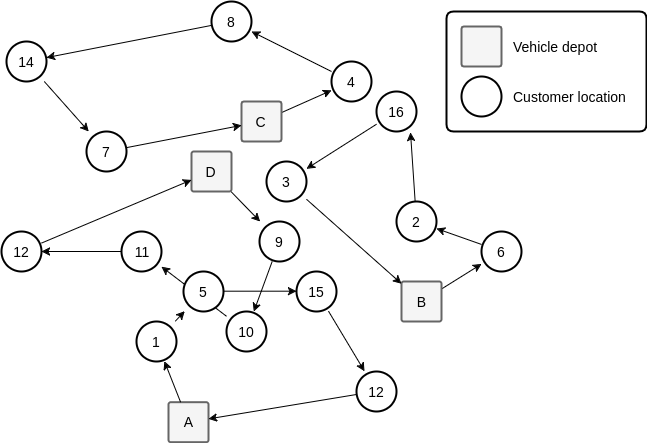
\includegraphics[width=9cm]{Resources/Images/result-mdvrp-illustration}
	\caption{Ilustrasi Rute yang Dihasilkan}
	\label{fig:result-mdvrp-illustration}
\end{figure}


Total \textit{cost} untuk masing-masing rute kemudian dihitung dengan melakukan penjumlahan seluruh waktu tempuh dan waktu pelayanan (\textit{service time}) dari lokasi yang dikunjungi. Pada contoh \autoref{fig:result-mdvrp-illustration}, total \textit{cost} dari setiap kendaraan adalah:

\begin{itemize}
	\item $TC_A$ = $C_{A-1}$ + $ST_5$ + $C_{1-5}$ + $ST_5$ + $C_{5-15}$ + $ST_15$ + $C_{15-12}$ + $ST_12$ + $C_{12-A}$
	\item $TC_B$ = $C_{B-6}$ + $ST_6$ + $C_{6-2}$ + $ST_2$ + $C_{2-16}$ + $ST_16$ + $C_{16-3}$ + $ST_3$ + $C_{3-B}$
	\item $TC_C$ = $C_{C-4}$ + $ST_4$ + $C_{4-8}$ + $ST_8$ + $C_{8-14}$ + $ST_14$ + $C_{14-7}$ + $ST_7$ + $C_{7-C}$
	\item $TC_D$ = $C_{D-9}$ + $ST_9$ + $C_{9-10}$ + $ST_10$ + $C_{10-11}$ + $ST_11$ + $C_{11-12}$ + $ST_12$ + $C_{12-D}$
\end{itemize}
dimana TC adalah \textit{total cost}, C adalah \textit{transport cost} yang merupakan waktu tempuh, dan ST adalah \textit{service time}.


\textbf{\textit{Metric}} yang digunakan untuk mengukur perbandingan antar pengujian adalah standar deviasi dari seluruh rute yang dihasilkan oleh sistem usulan maupun sistem pembanding. Standar deviasi dipilih sebagai \textit{metric} karena lebih merepresentasikan kondisi pencacahan yang sebenarnya, dimana semakin kecil variasi waktu antar petugas, semakin merata beban tugas yang berimbas pada penyelesaian pencacahan secara keseluruhan akan lebih cepat. Sistem yang lebih baik akan menghasilkan standar deviasi yang lebih kecil.


%-----------------------------------------------------------------------------%
\subsection{Skenario dan Hasil Pengujian}
%-----------------------------------------------------------------------------%
Pengujian dilakukan dengan beberapa skenario untuk memastikan bahwa program dapat bekerja dengan baik pada kondisi yang berbeda-beda. Mekanisme \textit{setup} serta skenario yang digunakan dalam pengujian akan dijabarkan pada pengujian dan skenario yang diujicobakan pada penelitian ini beserta hasilnya dijelaskan pada \autoref{ssec:broker-setup} hingga \autoref{sssec:test-delay-service-time}.


%-----------------------------------------------------------------------------%
\subsubsection{\textit{Message Broker Setup}}
\label{ssec:broker-setup}
%-----------------------------------------------------------------------------%
Seluruh skenario dalam pengujian ini akan menggunakan Redis sebagai \textit{message broker}. Redis merupakan \textit{in-memory data structure store} yang dapat digunakan sebagai \textit{database}, \textit{cache}, dan \textit{message broker} \citep{redis_introduction_2017}. Redis mempunyai \textit{feature} Redis Cluster, sehingga dapat dengan mudah disusun menjadi \textit{distributed message broker}. Selain itu, Redis \textit{client} tersedia dalam sebagian besar bahasa pemrograman \citep{redis_clients_2017}, sehingga memungkinkan pemilihan bahasa pemrograman dalam implementasi sistem secara lebih fleksibel.


Pada penelitian ini, Redis Cluster dikonfigurasi dengan menggunakan 6 (enam) buah \textit{nodes}, 3 (tiga) node digunakan sebagai \textit{master} dan sisanya sebagai \textit{slave}. Konfigurasi Redis Cluster pada setiap node diilustrasikan pada Kode \autoref{lst:redis_conf}. Dalam konteks Redis, master dapat dianggap sebagai partisi, dan slave dianggap sebagai replikasi dari master. Seluruh node, baik master maupun slave dapat digunakan sebagai \textit{entrypoint} dimana client terkoneksi.


\begin{listing}[!]
	\caption{Konfigurasi Redis Cluster}
	\label{lst:redis_conf}
	\begin{minted}[showspaces=false,breaklines=true]{java}
cluster-enabled yes
cluster-node-timeout 5000
cluster-config-file nodes.conf
appendonly yes
dir /data
	\end{minted}
\end{listing}


\textit{Nodes} Redis yang telah dikonfigurasi dan dijalankan, dapat digunakan untuk membuat cluster dengan memanfaatkan  \textit{script} \textbf{redis-trib.rb} yang telah disediakan oleh Redis. \textit{Command} yang digunakan dalam pembuatan cluster serta  \textit{response} yang diperoleh diilustrasikan pada Kode \autoref{lst:redis_trib_cluster} dan \autoref{lst:redis_trib_cluster_response}. \autoref{fig:test-flowchart-normal-global-broker} 
menyajikan \textit{flowchart} subsistem \textit{message broker setup}. 


\begin{listing}[!]
	\caption{Pembuatan Redis Cluster}
	\label{lst:redis_trib_cluster}
	\begin{minted}[showspaces=false,breaklines=true]{java}
/redis-trib.rb create --replicas 1 172.17.0.3 172.17.0.4 172.17.0.5 172.17.0.6 172.17.0.7 172.17.0.8
	\end{minted}
\end{listing}


\begin{listing}[!]
	\caption{Respon Pembuatan Redis Cluster}
	\label{lst:redis_trib_cluster_response}
	\begin{minted}[showspaces=false,breaklines=true]{java}
Creating cluster
Performing hash slots allocation on 6 nodes...
Using 3 masters:
172.17.0.3:6379
172.17.0.4:6379
172.17.0.5:6379
Adding replica 172.17.0.6:6379 to 172.17.0.3:6379
Adding replica 172.17.0.7:6379 to 172.17.0.4:6379
Adding replica 172.17.0.8:6379 to 172.17.0.5:6379
M: 2f0c681921fe52900a6774fb2cc808a8c4e69216 172.17.0.3:6379
slots:0-5460 (5461 slots) master
M: 41a343142847138301ceeb710206284a50bb44a0 172.17.0.4:6379
slots:5461-10922 (5462 slots) master
M: 88ae20b9e75dd5aa58973f13aa89479f52cedfd3 172.17.0.5:6379
slots:10923-16383 (5461 slots) master
S: c5f6764d82ed10793c0c81e54830b4f68b1eacd7 172.17.0.6:6379
replicates 2f0c681921fe52900a6774fb2cc808a8c4e69216
S: 5906f61963d4a5a45478736d976b79db4280b3c7 172.17.0.7:6379
replicates 41a343142847138301ceeb710206284a50bb44a0
S: 635ed817b134b5d14bffd61fe9089867037fee8c 172.17.0.8:6379
replicates 88ae20b9e75dd5aa58973f13aa89479f52cedfd3
Can I set the above configuration? (type 'yes' to accept): yes
Nodes configuration updated
Assign a different config epoch to each node
Sending CLUSTER MEET messages to join the cluster
Waiting for the cluster to join...
Performing Cluster Check (using node 172.17.0.3:6379)
M: 2f0c681921fe52900a6774fb2cc808a8c4e69216 172.17.0.3:6379
slots:0-5460 (5461 slots) master
1 additional replica(s)
M: 88ae20b9e75dd5aa58973f13aa89479f52cedfd3 172.17.0.5:6379
slots:10923-16383 (5461 slots) master
1 additional replica(s)
S: c5f6764d82ed10793c0c81e54830b4f68b1eacd7 172.17.0.6:6379
slots: (0 slots) slave
replicates 2f0c681921fe52900a6774fb2cc808a8c4e69216
M: 41a343142847138301ceeb710206284a50bb44a0 172.17.0.4:6379
slots:5461-10922 (5462 slots) master
1 additional replica(s)
S: 635ed817b134b5d14bffd61fe9089867037fee8c 172.17.0.8:6379
slots: (0 slots) slave
replicates 88ae20b9e75dd5aa58973f13aa89479f52cedfd3
S: 5906f61963d4a5a45478736d976b79db4280b3c7 172.17.0.7:6379
slots: (0 slots) slave
replicates 41a343142847138301ceeb710206284a50bb44a0
[OK] All nodes agree about slots configuration.
Check for open slots...
Check slots coverage...
[OK] All 16384 slots covered.
	\end{minted}
\end{listing}


%-----------------------------------------------------------------------------%
\subsubsection{\textit{Publisher Setup}}
%-----------------------------------------------------------------------------%
Publisher dikonfigurasi dan dijalankan pada lingkungan yang telah didefinisikan pada \autoref{ssec:test-environment}, sesuai dengan alur yang digambarkan pada \autoref{fig:test-flowchart-normal-global-publisher}. Format penggunaan Publisher diilustrasikan pada \autoref{lst:publisher-usage}.


\begin{listing}[!]
	\caption{Format penggunaan Publisher}
	\label{lst:publisher-usage}
	\begin{minted}[showspaces=false,breaklines=true]{bash}
Usage: mdvrp-redis-producer [options]

Run location recommendation server

Options:
-h, --help            show this help message and exit
-b BIN, --coes-bin=BIN
Binary of CoES MDVRP library
-D D, --data=D        Data problem file
-C C, --cost-file=C   Cost matrix file
-O O, --output-dir=O  Output directory
-t, --use-timestamp   Append timestamp to output directory
-B B, --broker-url=B  Redis broker URL
-X X, --solver-execution-time=X
VRP Solver execution time
	\end{minted}
\end{listing}


%-----------------------------------------------------------------------------%
\subsubsection{\textit{Subscriber Setup}}
%-----------------------------------------------------------------------------%
Pengujian memerlukan sebuah program tambahan yang berperan sebagai pencacah/\textit{subscriber}. Alur kerja dari masing-masing \textit{subscriber} (\autoref{fig:test-flowchart-normal-global-subscriber}) adalah sebagai berikut:


\begin{enumerate}
	\item Lakukan \textit{subscription} (pengiriman \textit{request}) pada \textit{message broker} dengan topik \textit{current location} dari \textit{subscriber}. 
	\item Sebuat \textit{reply} akan diterima dari \textit{publisher} yang dikirim melalui \textit{message broker} berupa lokasi pencacahan berikutnya yang akan dikunjungi. 
	\item Lakukan perjalanan ke lokasi yang akan dikunjungi yang disimulasikan dengan `\textit{sleep}'
	\item Setelah tiba di lokasi, simpan \textit{current location} pada \textit{shared memory} 
	\item Lakukan pencacahan yang disimulasikan dengan \textit{sleep}, 
	\item Ulangi proses dari langkah pertama.
\end{enumerate}


\begin{figure}[!]
	\centering
	\begin{subfigure}[t]{0.3\textwidth}
		\centering
		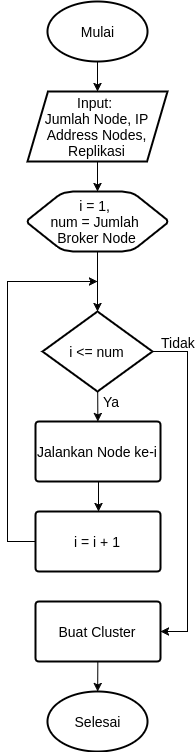
\includegraphics[width=\textwidth]{Resources/Images/test-flowchart-normal-global-broker}
		\caption{\textit{Flowchart Message Broker}}
		\label{fig:test-flowchart-normal-global-broker}
	\end{subfigure}%
	~
	\begin{subfigure}[t]{0.39\textwidth}
		\centering
		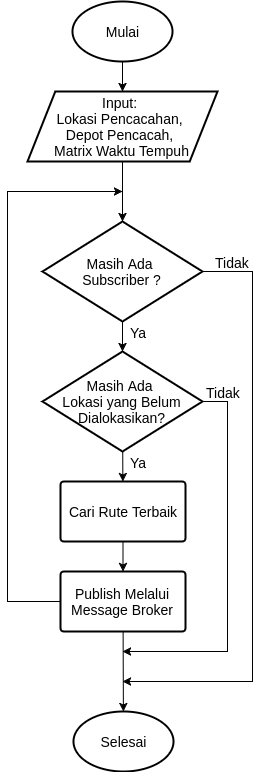
\includegraphics[width=\textwidth]{Resources/Images/test-flowchart-normal-global-publisher}
		\caption{\textit{Flowchart Publisher}}
		\label{fig:test-flowchart-normal-global-publisher}
	\end{subfigure}%
	~
	\begin{subfigure}[t]{0.31\textwidth}
		\centering
		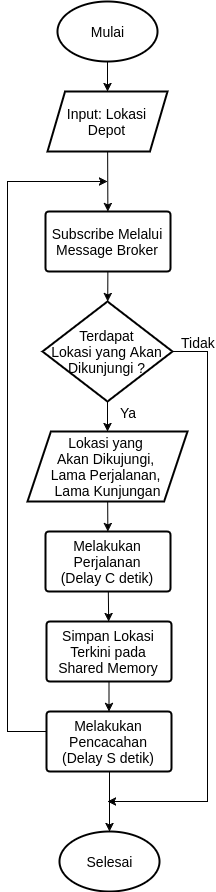
\includegraphics[width=\textwidth]{Resources/Images/test-flowchart-normal-global-subscriber}
		\caption{\textit{Flowchart Subscriber}}
		\label{fig:test-flowchart-normal-global-subscriber}
	\end{subfigure}
	\caption{\textit{Flowchart} Subsistem pada Pengujian}
	\label{fig:test-flowchart-normal-global}
\end{figure}


%-----------------------------------------------------------------------------%
\subsubsection{Pengujian Tanpa \textit{Service Time}}
%-----------------------------------------------------------------------------%
Pengujian ini bertujuan membandingkan keakuratan sistem dalam memproses data tanpa melibatkan \textit{service time} dari \textit{customer}-nya. Data \textit{subscriber} dan \textit{customer} di-\textit{generate} secara random, baik dalam hal jumlah maupun koordinat lokasi. Data yang digunakan diperoleh dari \textit{instance} Cordeau P01 sampai P10, dengan masing-masing komposisi sebagai berikut:


\begin{enumerate}
	\item Instance P01 terdiri dari 50 \textit{customer} dan 5 \textit{vehicle},
	\item Instance P02 terdiri dari 50 \textit{customer} dan 4 \textit{vehicle}, 
	\item Instance P03 terdiri dari 75 \textit{customer} dan 5 \textit{vehicle}, 
	\item Instance P04 terdiri dari 100 \textit{customer} dan 2 \textit{vehicle}, 
	\item Instance P05 terdiri dari 100 \textit{customer} dan 2 \textit{vehicle}, 
	\item Instance P06 terdiri dari 100 \textit{customer} dan 3 \textit{vehicle}, 
	\item Instance P07 terdiri dari 100 \textit{customer} dan 4 \textit{vehicle}, 
	\item Instance P08 terdiri dari 249 \textit{customer} dan 2 \textit{vehicle}, 
	\item Instance P09 terdiri dari 249 \textit{customer} dan 3 \textit{vehicle}, 
	\item Instance P10 terdiri dari 249 \textit{customer} dan 4 \textit{vehicle}.
\end{enumerate}
Terminologi \textit{vehicle} dan \textit{customer} pada data Cordeau analog dengan pencacah dan lokasi pencacahan pada permasalahan rekomendasi lokasi pencacahan.


Dari hasil simulasi, diperoleh rute untuk masing-masing \textit{instance} Cordeau sebagaimana digambarkan pada \hyperref[ch:test_result_cordeau_notw]{Lampiran 1}. Kemudian dari seluruh rute yang diperoleh, dikalkulasi \textit{total time} untuk masing-masing rute, sebagaimana cara yang dijelaskan pada \autoref{sssec:metric}. 

Hasil pengujian pada \autoref{tbl:test_result_10_cordeau} menunjukkan bahwa sistem pembanding (CoEAs + MDVRP) lebih unggul dari \textbf{segi total waktu pencacahan}, dimana 8 dari 10 \textit{instance} yang diujikan memiliki total waktu yang lebih kecil jika diproses dengan sistem pembanding. Namun, dari segi \textbf{standar deviasi}, sistem usulan (CoEAs + MDVRP + \textit{publish/subscribe}) jauh mengungguli sistem pembanding, dimana 8 dari 10 \textit{instance} yang diujikan dengan sistem usulan menghasilkan standar deviasi yang lebih kecil dibandingkan standar deviasi dari sistem pembanding. 

Standar deviasi yang kecil berarti terdapat waktu penyelesaian tugas antar pencacah yang hampir setara, sehingga seluruh kegiatan pencacahan dapat selesai pada waktu yang hampir bersamaan. Hal ini berbanding terbalik dengan sistem pembanding yang walaupun memiliki total waktu yang lebih kecil, namun standar deviasinya lebih besar. Akibatnya terdapat bias dalam waktu penyelesaian pekerjaan antar petugas yang menyebabkan terjadinya selisih waktu penyelesaian yang cukup besar. Hal ini berdampak pada semakin lamanya total waktu kegiatan pencacahan secara keseluruhan, karena terdapat `waktu tunggu' dimana BPS harus menunggu hingga seluruh pencacah menyelesaikan pekerjaannya. 


\autoref{fig:test_result_10_cordeau_total_time} dan \autoref{fig:test_result_10_cordeau_standard_deviation} menggambarkan perbandingan hasil pengujian dari 10 \textit{instance} Cordeau.


\begin{longtable}[!]{l|rrrr}
	\caption{Hasil Pengujian Tanpa \textit{Service Time} pada Data Cordeau}
	\label{tbl:test_result_10_cordeau}\\
	\toprule
	\textit{Instance} & \MyHead{2.5cm}{Total Waktu CoES MDVRP (det)} & \MyHead{2.5cm}{Total Waktu CoES MDVRP + Pub/Sub (det)} & \MyHead{2.5cm}{Stdev Waktu CoES MDVRP (det)} & \MyHead{2.5cm}{Stdev Waktu CoES MDVRP + Pub/Sub (det)} \\ 
	\midrule
	\endfirsthead
	\toprule
	\textit{Instance} & \MyHead{2.5cm}{Total Waktu CoES MDVRP (det)} & \MyHead{2.5cm}{Total Waktu CoES MDVRP + Pub/Sub (det)} & \MyHead{2.5cm}{Stdev Waktu CoES MDVRP (det)} & \MyHead{2.5cm}{Stdev Waktu CoES MDVRP + Pub/Sub (det)} \\ 
	\midrule
	\endhead
	\bottomrule
	\endfoot
	p01 & \textbf{454.91} & 573.77 & 27.24 & \textbf{20.84} \\
	p02 & \textbf{462.61} & 550.61 & 25.90 & \textbf{13.32} \\
	p03 & \textbf{590.98} & 696.93 & 32.47 & \textbf{20.09} \\
	p04 & 1.321.89 & \textbf{1.264.53} & 199.16 & \textbf{16.10} \\
	p05 & \textbf{1.039.68} & 1.520.53 & 76.61 & \textbf{1.09} \\
	p06 & \textbf{679.11} & 1.160.76 & 57.15 & \textbf{48.82} \\
	p07 & \textbf{782.41} & 973.72 & \textbf{29.08} & 67.27 \\
	p08 & 8.353.76 & \textbf{6.172.66} & 1.962.81 & \textbf{228.95} \\
	p09 & \textbf{2.669.29} & 4.275.12 & 208.99 & \textbf{117.76} \\
	p10 & \textbf{2.692.06} & 4.132.31 & \textbf{130.08} & 200.31 \\
\end{longtable}


\begin{figure}[H]
	\centering
	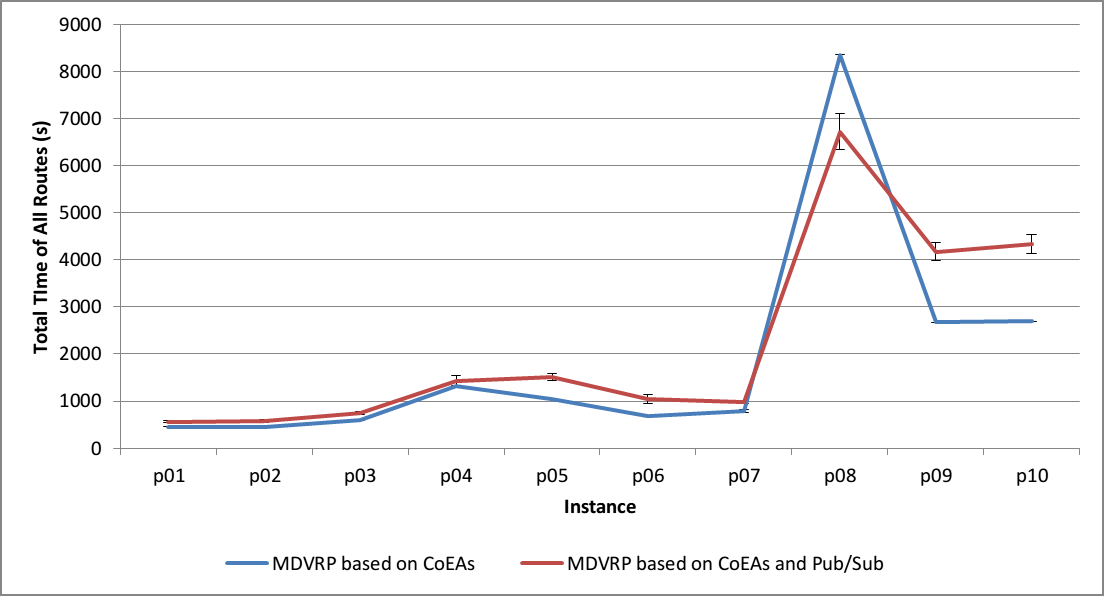
\includegraphics[width=\textwidth]{Resources/Images/test_result_10_cordeau_total_time}
	\caption{Perbandingan Waktu Total dari 10 \textit{Instance} Cordeau}
	\label{fig:test_result_10_cordeau_total_time}
\end{figure}


\begin{figure}[H]
	\centering
	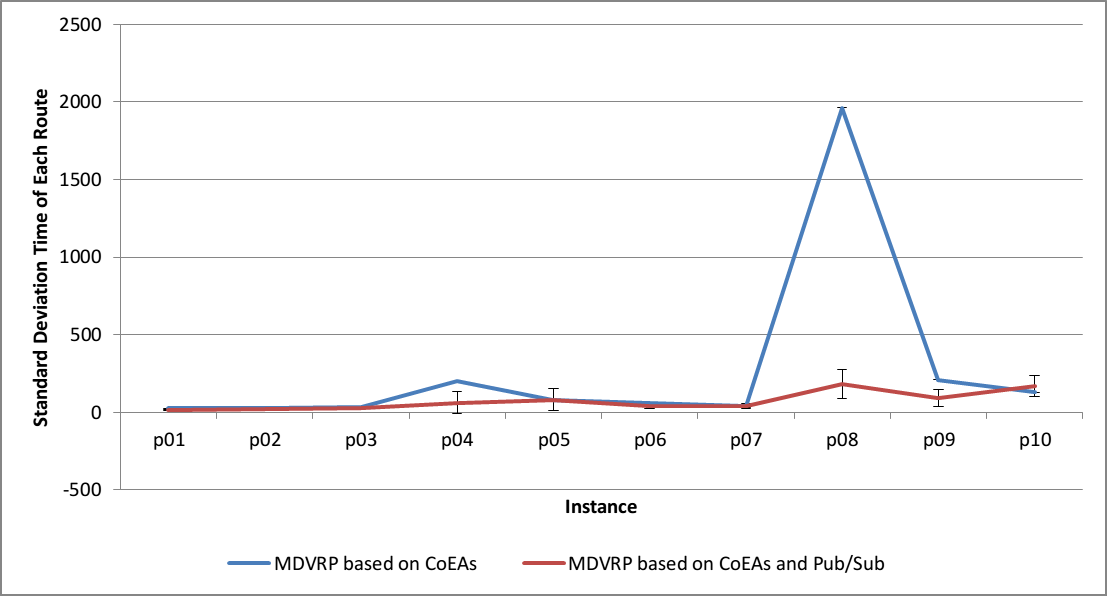
\includegraphics[width=\textwidth]{Resources/Images/test_result_10_cordeau_standard_deviation}
	\caption{Perbandingan Standar Deviasi Waktu dari 10 \textit{Instance} Cordeau}
	\label{fig:test_result_10_cordeau_standard_deviation}
\end{figure}


%-----------------------------------------------------------------------------%
\subsubsection{Pengujian Kondisi Normal dengan \textit{Service Time}}
\label{ssec:test-normal-service-time}
%-----------------------------------------------------------------------------%
Skenario pengujian kondisi normal dimaksudkan untuk membandingkan sistem yang dijalankan pada kondisi normal, dimana tidak ada sesuatupun yang menyebabkan penundaaan. Pengujian kondisi ini dilakukan untuk masing-masing data Cordeau (P01 sampai P10) dan data lapangan. 


Data \textit{service time} digenerate secara random dengan mengikuti komposisi dari \citep{sudman_time_1965}, yaitu:
\begin{enumerate}
	\item 21 persen dari total waktu digunakan untuk perpindahan antar segmen, 
	\item 15 persen dari total waktu digunakan untuk perpindahan antar rumah tangga dalam segmen, 
	\item 37 persen dari total waktu digunakan untuk wawancara seluruh responden, dan 
	\item 27 persen untuk hal-hal yang lain, seperti pengenalan wilayah dan perbaikan data.
\end{enumerate}
\textit{Service time} merupakan gabungan dari waktu perpindahan antar rumah tangga dan waktu wawancara. Meskipun komposisi waktu \citep{sudman_time_1965} dinilai kurang relevan, akan tetapi masih dapat digunakan sebagai dasar untuk men-\textit{generate} \textit{service time}. Adapun penggunaan komposisi waktu yang lebih relevan terdapat pada \autoref{sssec:test-delay-service-time}.


Berikut adalah komposisi dari masing-masing \textit{instance} Cordeau:
\begin{enumerate}
	\item Instance P01 terdiri dari 50 \textit{customer} dan 5 \textit{vehicle}, lama wawancara 27.58 menit dengan standar deviasi 12.13 menit.
	\item Instance P02 terdiri dari 50 \textit{customer} dan 4 \textit{vehicle}, lama wawancara 27.58 menit dengan standar deviasi 12.13 menit.
	\item Instance P03 terdiri dari 75 \textit{customer} dan 5 \textit{vehicle}, lama wawancara 27.58 menit dengan standar deviasi 12.13 menit.
	\item Instance P04 terdiri dari 100 \textit{customer} dan 2 \textit{vehicle}, lama wawancara 27.58 menit dengan standar deviasi 12.13 menit.
	\item Instance P05 terdiri dari 100 \textit{customer} dan 2 \textit{vehicle}, lama wawancara 27.58 menit dengan standar deviasi 12.13 menit.
	\item Instance P06 terdiri dari 100 \textit{customer} dan 3 \textit{vehicle}, lama wawancara 27.58 menit dengan standar deviasi 12.13 menit.
	\item Instance P07 terdiri dari 100 \textit{customer} dan 4 \textit{vehicle}, lama wawancara 27.58 menit dengan standar deviasi 12.13 menit.
	\item Instance P08 terdiri dari 249 \textit{customer} dan 2 \textit{vehicle}, lama wawancara 27.58 menit dengan standar deviasi 12.13 menit.
	\item Instance P09 terdiri dari 249 \textit{customer} dan 3 \textit{vehicle}, lama wawancara 27.58 menit dengan standar deviasi 12.13 menit.
	\item Instance P10 terdiri dari 249 \textit{customer} dan 4 \textit{vehicle}, lama wawancara 27.58 menit dengan standar deviasi 12.13 menit.
\end{enumerate}
Adapun data lapangan memiliki komposisi sebagai berikut:
\begin{enumerate}
	\item Instance TW1 terdiri dari 182 \textit{customer} dan 15 \textit{vehicle}, lama wawancara 27.58 menit dengan standar deviasi 4,13 menit.
	\item Instance TW2 terdiri dari 182 \textit{customer} dan 15 \textit{vehicle}, lama wawancara 71.58 menit dengan standar deviasi 12.16 menit.
	\item Instance TW3 terdiri dari 182 \textit{customer} dan 15 \textit{vehicle}, lama wawancara 27.35 menit dengan standar deviasi 25.34 menit.
	\item Instance TW4 terdiri dari 182 \textit{customer} dan 15 \textit{vehicle}, lama wawancara 71.58 menit dengan standar deviasi 56.87 menit.
\end{enumerate}


Dari hasil simulasi, diperoleh rute untuk masing-masing \textit{instance} Cordeau sebagaimana digambarkan pada \hyperref[ch:test_result_cordeau_notw]{Lampiran 1}. Kemudian dari seluruh rute yang diperoleh, dikalkulasi \textit{total time} untuk masing-masing rute, sebagaimana cara yang dijelaskan pada \autoref{sssec:metric}. Berdasarkan \autoref{tbl:test_result_10_cordeau_tw}, diperoleh hasil bahwasannya dengan menggunakan sistem usulan, seluruh \textit{instance} menghasilkan \textbf{total waktu} yang lebih kecil. Sementara dari sisi \textbf{standar deviasi}, diperoleh hasil bahwa seluruh \textit{instance} menghasilkan standar deviasi yang lebih kecil. Hal ini berarti, program usulan yang berupa MDVRP berbasis CoEAs dan mekansime \textit{publish/subscribe} lebih efisien karena beban tugas yang lebih merata antar petugas menyebabkan total waktu seluruh kegiatan menjadi lebih pendek dibandingkan sistem pembanding. 


\begin{longtable}[!]{l|rrrr}
	\caption{Hasil Pengujian Kondisi Normal Pada Data Cordeau Dengan \textit{Service Time}}
	\label{tbl:test_result_10_cordeau_tw}\\
	\toprule
	\textit{Instance} & \MyHead{2.5cm}{Total Waktu CoES MDVRP (det)} & \MyHead{2.5cm}{Total Waktu CoES MDVRP + Pub/Sub (det)} & \MyHead{2.5cm}{Stdev Waktu CoES MDVRP (det)} & \MyHead{2.5cm}{Stdev Waktu CoES MDVRP + Pub/Sub (det)} \\ 
	\midrule
	\endfirsthead
	\toprule
	\textit{Instance} & \MyHead{2.5cm}{Total Waktu CoES MDVRP (det)} & \MyHead{2.5cm}{Total Waktu CoES MDVRP + Pub/Sub (det)} & \MyHead{2.5cm}{Stdev Waktu CoES MDVRP (det)} & \MyHead{2.5cm}{Stdev Waktu CoES MDVRP + Pub/Sub (det)} \\ 
	\midrule
	\endhead
	\bottomrule
	\endfoot
	p01 & \textbf{824,513.17} & 824,649.98 & 44,165.10 & \textbf{12,539.43} \\
	p02 & \textbf{805,990.03} & 806,090.97 & 37,666.96 & \textbf{12,322.08} \\
	p03 & \textbf{1,256,883.28} & 1,257,044.56 & 57,486.44 & \textbf{13,271.86} \\
	p04 & \textbf{1,642,834.05} & 1,643,051.50 & 148,762.94 & \textbf{4,719.26} \\
	p05 & \textbf{1,654,118.92} & 1,654,511.94 & 154,028.63 & \textbf{22,469.85} \\
	p06 & \textbf{1,634,803.49} & 1,635,193.62 & 103,266.13 & \textbf{10,160.24} \\
	p07 & \textbf{1,639,779.18} & 1,639,996.92 & 81,233.61 & \textbf{5,492.17} \\
	p08 &  &  &  &  \\
	p09 &  &  &  &  \\
	p10 & \textbf{4,115,466.02} & 4,117,128.75 & 223,253.75 & \textbf{13,662.48} \\
\end{longtable}


Sementara itu, pada pengujian dengan menggunakan data lapangan, diperoleh hasil sebagaimana digambarkan pada \hyperref[ch:test_result_cordeau_notw]{Lampiran 1}. Kemudian dari seluruh rute yang diperoleh, dikalkulasi \textit{total time} untuk masing-masing rute, sebagaimana cara yang dijelaskan pada \autoref{sssec:metric}. Berdasarkan \autoref{tbl:test_result_4_real_tw}, diperoleh hasil bahwasannya \textbf{total waktu} yang dihasilkan dengan menggunakan sistem usulan keseluruhannya lebih besar dibandingkan dengan menggunakan aplikasi pembanding. Sementara dari sisi \textbf{standar deviasi}, keseluruhan \textit{instance} menghasilkan standar deviasi yang lebih kecil. Hal ini kembali membuktikan efisiensi sistem usulan dibandingkan sistem pembanding karena beban tugas yang lebih merata antar petugas menyebabkan total waktu seluruh kegiatan menjadi lebih pendek. 

\autoref{fig:test_result_4_real_tw_total_time} dan \autoref{fig:test_result_4_real_tw_standard_deviation} menggambarkan perbandingan hasil pengujian dari 4 \textit{instance} data lapangan.


\begin{longtable}[!]{l|rrrr}
	\caption{Hasil Pengujian Kondisi Normal Pada Data Lapangan Dengan \textit{Service Time}}
	\label{tbl:test_result_4_real_tw}\\
	\toprule
	\textit{Instance} & \MyHead{2.5cm}{Total Waktu CoES MDVRP (det)} & \MyHead{2.5cm}{Total Waktu CoES MDVRP + Pub/Sub (det)} & \MyHead{2.5cm}{Stdev Waktu CoES MDVRP (det)} & \MyHead{2.5cm}{Stdev Waktu CoES MDVRP + Pub/Sub (det)} \\ 
	\midrule
	\endfirsthead
	\toprule
	\textit{Instance} & \MyHead{2.5cm}{Total Waktu CoES MDVRP (det)} & \MyHead{2.5cm}{Total Waktu CoES MDVRP + Pub/Sub (det)} & \MyHead{2.5cm}{Stdev Waktu CoES MDVRP (det)} & \MyHead{2.5cm}{Stdev Waktu CoES MDVRP + Pub/Sub (det)} \\ 
	\midrule
	\endhead
	\bottomrule
	\endfoot
	tw01 & \textbf{3,119,907.52} & 3,574,996.52 & 82,529.44 & \textbf{24,134.25} \\
	tw02 & \textbf{7,892,350.51} & 8,136,451.51 & 210,200.68 & \textbf{17,801.33} \\
	tw03 & \textbf{3,166,715.70} & 3,346,362.70 & 83,961.70 & \textbf{22,296.01} \\
	tw04 & \textbf{7,868,523.23} & 8,060,837.23 & 205,597.64 & \textbf{25,430.96} \\
\end{longtable}


\begin{figure}[H]
	\centering
	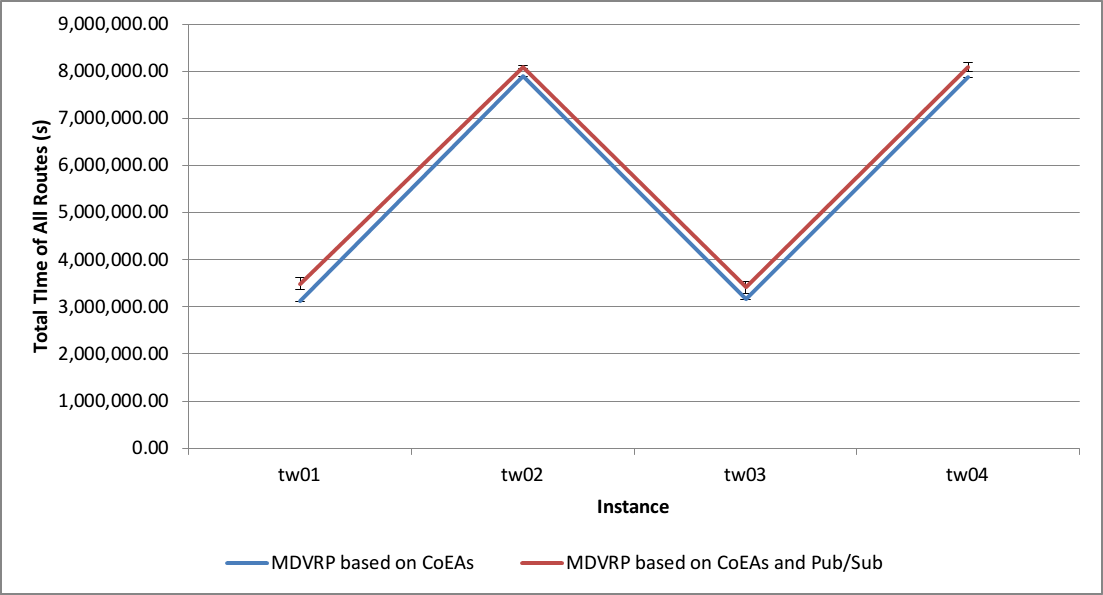
\includegraphics[width=\textwidth]{Resources/Images/test_result_4_real_tw_total_time}
	\caption{Perbandingan Waktu Total Pengujian Kondisi Normal Pada Data Lapangan Dengan \textit{Service Time}}
	\label{fig:test_result_4_real_tw_total_time}
\end{figure}


\begin{figure}[H]
	\centering
	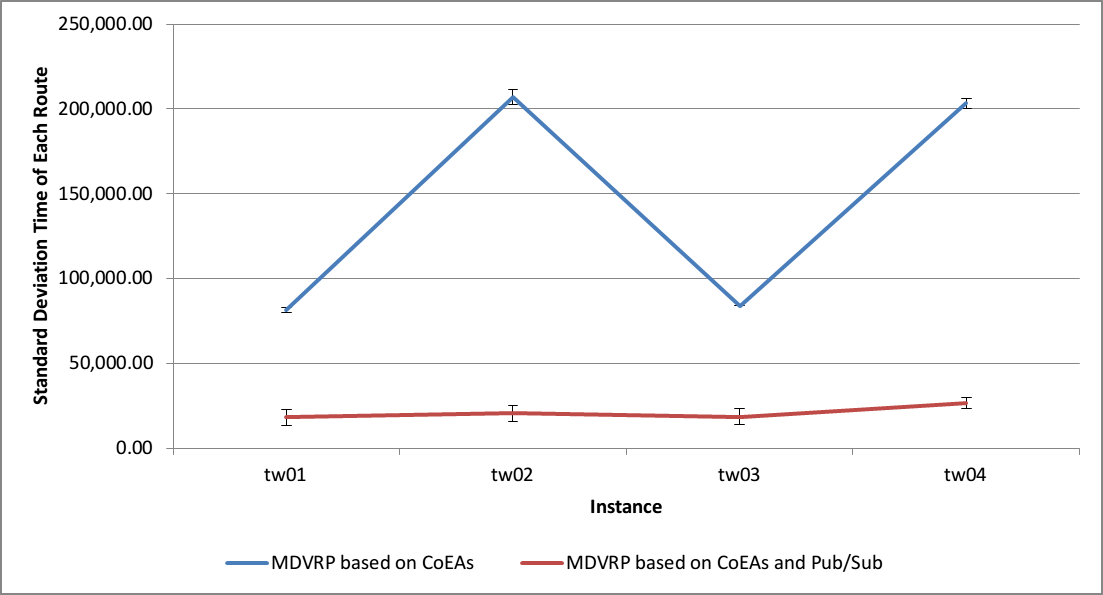
\includegraphics[width=\textwidth]{Resources/Images/test_result_4_real_tw_standard_deviation}
	\caption{Perbandingan Standar Deviasi Waktu Pengujian Kondisi Normal Pada Data Lapangan Dengan \textit{Service Time}}
	\label{fig:test_result_4_real_tw_standard_deviation}
\end{figure}


%Setelah simulasi dilakukan, dari seluruh rute yang diperoleh kemudian dikalkulasi \textit{total time} untuk masing-masing rute, sebagaimana cara yang dijelaskan pada \autoref{sssec:metric}. Selain itu juga sebuah grafik dibuat untuk memberikan ilustrasi rute pada masing-masing program pembanding dan sistem usulan.
%
%
%Pada pengujian dengan dataset Cordeau, diperoleh hasil sebagaimana \autoref{tbl:test_result_normal_cordeau_coes} untuk algoritma MDVRP berbasis CoEAs tanpa mekanisme Publish/Subscribe, dan \autoref{tbl:test_result_normal_cordeau_pubsub_coes} untuk algoritma MDVRP berbasis CoEAs dengan mekanisme Publish/Subscribe. Sementara \autoref{fig:test_result_normal_cordeau_comparison} menggambarkan rute yang diperoleh untuk masing-masing program.
%
%
%Berdasarkan \autoref{tbl:test_result_normal_cordeau_comparison}, diperoleh hasil bahwasannya \textbf{total waktu} yang diperoleh dengan menggunakan sistem MDVRP berbasis CoEAs dan Publish/Subscribe lebih buruk 6,25 persen  dibandingkan dengan program usulan. Akan tetapi dari sisi \textbf{standar deviasi} dari keseluruhan rute diperoleh hasil metode CoEAs yang dikombinasikan dengan Publish/Subscribe menghasilkan angka yang lebih baik 68.83 persen, yang artinya total waktu dari seluruh rute lebih merata.
%
%
%\begin{longtable}[!]{lp{8cm}r}
%	\caption{Hasil Pengujian Kondisi Normal (Cordeau), MDVRP berbasis CoEAs}
%	\label{tbl:test_result_normal_cordeau_coes}\\
%	\toprule
%		\textit{Vehicle} & Rute & Waktu Total\\ 
%	\midrule
%	\endfirsthead
%	\toprule
%		\textit{Vehicle} & Rute & Waktu Total\\ 
%	\midrule
%	\endhead
%	\bottomrule
%	\endfoot
%		51 & 42-19-40-41-13-18-4-17-37-15-44 & 194,775.99 \\
%		52 & 27-48-6-14-25-24-43-23-7-26-8-1-32-11-12-47-46 & 312,308.79 \\
%		53 & 9-38-5-45-33-39-10-30-34-50-49 & 198,178.68 \\
%		54 & 29-21-16-2-22-28-31-3-20-35-36 & 199,754.93 \\
%\end{longtable}
%
%
%\begin{longtable}[!]{lp{8cm}r}
%	\caption{Hasil Pengujian Kondisi Normal (Cordeau), MDVRP berbasis CoEAs dan Publish/Subscribe}
%	\label{tbl:test_result_normal_cordeau_pubsub_coes}\\
%	\toprule
%		\textit{Vehicle} & Rute & Waktu Total\\ 
%	\midrule
%	\endfirsthead
%	\toprule
%		\textit{Vehicle} & Rute & Waktu Total\\ 
%	\midrule
%	\endhead
%	\bottomrule
%	\endfoot
%		51 & 42-19-44-40-45-33-15-37-39-30-17-25-43 & 234,931.69 \\
%		52 & 27-46-12-47-18-24-4-41-6-48-13-14-23 & 236,669.22 \\
%		53 & 9-50-34-49-5-10-38-11-16-2-32 & 199,526.52 \\
%		54 & 29-21-20-35-36-31-28-3-22-26-1-8-7 & 234,154.12 \\
%\end{longtable}
%
%
%\begin{longtable}[!]{lrr}
%	\caption{Komparasi Hasi Pengujian Kondisi Normal Dengan Data Cordeau}
%	\label{tbl:test_result_normal_cordeau_comparison}\\
%	\toprule
%		\textit{Parameter} & CoEAs MDVRP  & Pub/Sub CoEAS MDVRP\\ 
%	\midrule
%	\endfirsthead
%	\toprule
%		\textit{Parameter} & CoEAs MDVRP  & Pub/Sub CoEAS MDVRP\\ 
%	\midrule
%	\endhead
%	\bottomrule
%	\endfoot
%		Total Waktu & \textbf{905,018.39} & 905,281.55\\
%		Rata-rata & \textbf{226,254.60} & 226,320.39\\
%		Standar Deviasi & 49,715.99 & \textbf{15,496.22}\\
%\end{longtable}
%
%
%\begin{figure}[!]
%    \centering
%    \begin{subfigure}[t]{\textwidth}
%        \centering
%		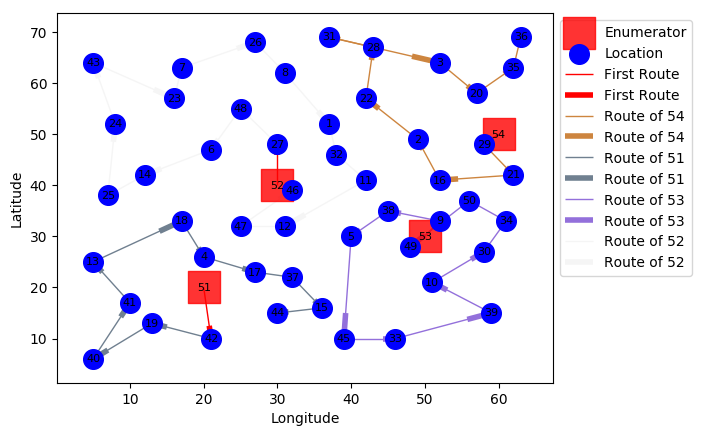
\includegraphics[width=\textwidth]{Resources/Images/test_result_normal_cordeau_p01_coes}
%		\caption{MDVRP berbasis CoEAs}
%		\label{fig:test_result_normal_cordeau_coes}
%    \end{subfigure}%
%    
%    \begin{subfigure}[t]{\textwidth}
%        \centering
%		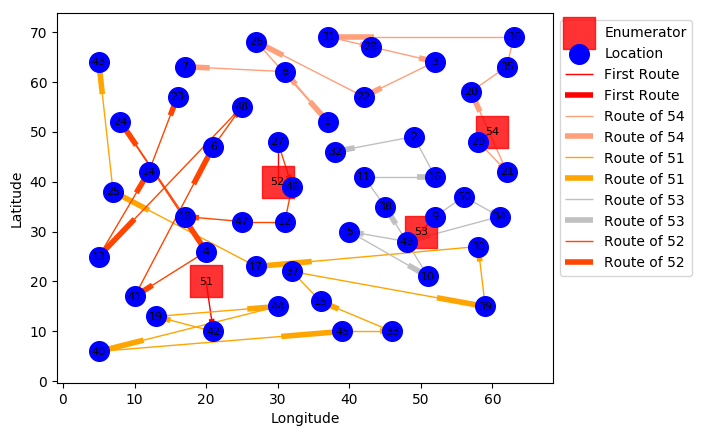
\includegraphics[width=\textwidth]{Resources/Images/test_result_normal_cordeau_p01_pubsub_coes}
%		\caption{MDVRP berbasis CoEAs dengan Publish/Subscribe}
%		\label{fig:test_result_normal_cordeau_pubsub_coes}
%    \end{subfigure}
%    \caption{Perbandingan Rute Hasil Pengujian Data Cordeau P01 Dengan \textit{Service Time}}
%    \label{fig:test_result_normal_cordeau_comparison}
%\end{figure}


%Sementara itu, pada pengujian dengan menggunakan data lapangan, diperoleh hasil sebagaimana \autoref{tbl:test_result_normal_field_coes} untuk algoritma MDVRP berbasis CoEAs tanpa mekanisme Publish/Subscribe, dan \autoref{tbl:test_result_normal_field_pubsub_coes} untuk algoritma MDVRP berbasis CoEAs dengan mekanisme Publish/Subscribe. Sementara \autoref{fig:test_result_normal_field_comparison} menggambarkan rute yang diperoleh untuk masing-masing program.
%
%
%Berdasarkan \autoref{tbl:test_result_normal_field_comparison}, diperoleh hasil bahwasannya \textbf{total waktu} yang diperoleh dengan menggunakan sistem MDVRP berbasis CoEAs dan Publish/Subscribe lebih buruk 8,25 persen  dibandingkan dengan program usulan. Akan tetapi dari sisi \textbf{standar deviasi} dari keseluruhan rute diperoleh hasil metode CoEAs yang dikombinasikan dengan Publish/Subscribe menghasilkan angka yang lebih baik 59,11 persen, yang artinya total waktu dari seluruh rute lebih merata.
%
%
%\begin{longtable}[!]{lp{8cm}r}
%	\caption{Hasil Pengujian Kondisi Normal (Lapangan), MDVRP berbasis CoEAs}
%	\label{tbl:test_result_normal_field_coes}\\
%	\toprule
%		\textit{Vehicle} & Rute & Waktu Total\\ 
%	\midrule
%	\endfirsthead
%	\toprule
%		\textit{Vehicle} & Rute & Waktu Total\\ 
%	\midrule
%	\endhead
%	\bottomrule
%	\endfoot
%		183 & 70-179-87-163-132-5-35-145-42 & 170,349.48 \\
%		184 & 159-174-60-36-99-98-171-50-9-7-8-152-111-51-40-172-38-134 & 331,759.24 \\
%		185 & 127-88-147-173-158-102-124-37-73-97 & 184,993.17 \\
%		186 & 157-93-94-146-155-123-162-161-156-89-138-77-44-109 & 254,089.65 \\
%		187 & 149-135-61-115-180-128 & 109,758.28 \\
%		188 & 165-47-92-78-69-108-120-136-41-71-55-4-33-178-160-1-151-3-2 & 355,614.60 \\
%		189 & 13-91-10-11-14-12-118-167-176 & 168,298.11 \\
%		190 & 104-141-63-117-45-131-81-177-170-67-49 & 193,952.81 \\
%		191 & 100-107-116-150-32-59 & 116,272.15 \\
%		192 & 86-168-143-95-76-103-53-52-166-65-54 & 211,842.84 \\
%		193 & 164-139-56-18-72-19-20-22-21-16-39-24-23-17-28-137-26-169-154-27-15-25-122-31 & 451,562.34 \\
%		194 & 142-126-30-58-110-46-82-80-148-106-96-84-68-182-34 & 275,108.47 \\
%		195 & 83-140-175-79-64-133-119-66-48 & 160,970.13 \\
%		196 & 29-112-113-43-121-74-90-125-153-6-181-62 & 220,804.42 \\
%		197 & 85-129-130-105-114-57-144-75-101 & 168,014.48 \\
%\end{longtable}
%
%
%\begin{longtable}[!]{lp{8cm}r}
%	\caption{Hasil Pengujian Kondisi Normal (Lapangan), MDVRP berbasis CoEAs dan Publish/Subscribe}
%	\label{tbl:test_result_normal_field_pubsub_coes}\\
%	\toprule
%		\textit{Vehicle} & Rute & Waktu Total\\ 
%	\midrule
%	\endfirsthead
%	\toprule
%		\textit{Vehicle} & Rute & Waktu Total\\ 
%	\midrule
%	\endhead
%	\bottomrule
%	\endfoot
%		183 & 70-179-87-163-132-38-51-68-96-139-58-7-30-8 & 277,856.33 \\
%		184 & 159-36-174-40-60-172-102-178-49-3-177-151 & 241,245.62 \\
%		185 & 127-88-147-173-158-1-124-37-67-73-170-97-77 & 253,954.73 \\
%		186 & 157-109-93-156-44-155-89-123-161-115-180-128-48-65-162 & 280,828.06 \\
%		187 & 149-135-61-94-146-138-120-136-12-71-176-33 & 269,049.32 \\
%		188 & 165-41-47-69-78-81-108-116-92-55-4-160-2 & 257,633.11 \\
%		189 & 13-91-10-11-131-167-118-14-126-110-148 & 229,909.92 \\
%		190 & 104-141-117-45-63-150-103-53-133-54-52-166 & 242,338.23 \\
%		191 & 100-107-32-59-76-64-66-171-119-9 & 246,133.18 \\
%		192 & 86-168-143-95-84-152-98-122-50-31-134-56-28 & 275,294.42 \\
%		193 & 164-24-182-106-111-99-39-22-72-21-19-16-20 & 258,783.38 \\
%		194 & 142-34-46-80-82-23-26-169-27-15-137-25-154-18-17 & 284,033.04 \\
%		195 & 83-140-175-79-121-75-43-5-125-153-6 & 220,121.19 \\
%		196 & 29-112-74-62-129-114-144 & 132,181.37 \\
%		197 & 85-130-101-57-105-113-181-35-90-42-145 & 207,356.29 \\
%\end{longtable}
%
%
%\begin{longtable}[!]{lrr}
%	\caption{Komparasi Hasi Pengujian Kondisi Normal Dengan Data Lapangan}
%	\label{tbl:test_result_normal_field_comparison}\\
%	\toprule
%	\textit{Parameter} & CoEAs MDVRP  & Pub/Sub CoEAS MDVRP\\ 
%	\midrule
%	\endfirsthead
%	\toprule
%	\textit{Parameter} & CoEAs MDVRP  & Pub/Sub CoEAS MDVRP\\ 
%	\midrule
%	\endhead
%	\bottomrule
%	\endfoot
%		Total Waktu & \textbf{3,373,390.19} & 3,676,718.19\\
%		Rata-rata & \textbf{224,892.68} & 245,114.55\\
%		Standar Deviasi & 91,123.23 & \textbf{37,261.85}\\
%\end{longtable}
%
%
%\begin{figure}[H]
%	\centering
%	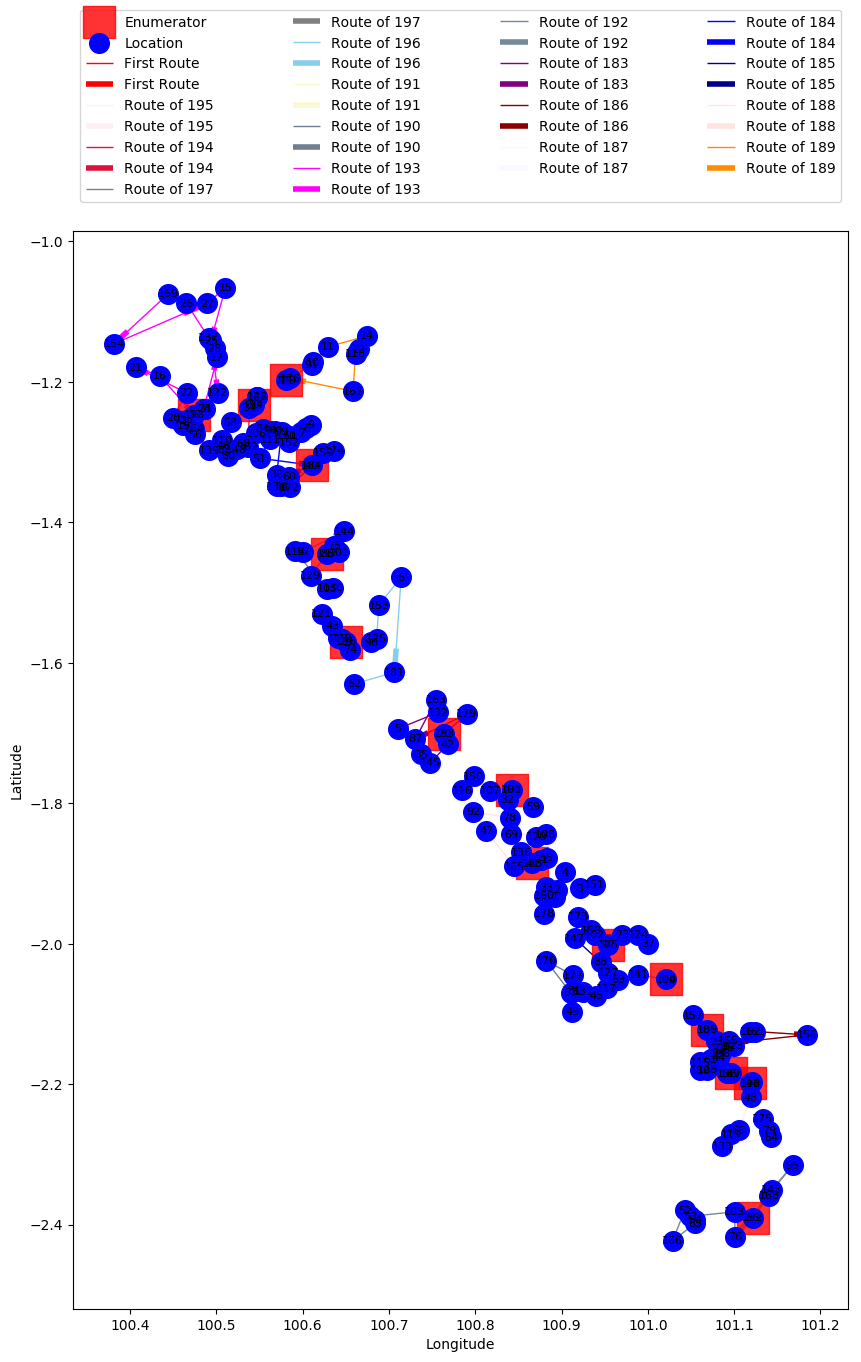
\includegraphics[width=\textwidth]{Resources/Images/test_result_normal_field_m15_n182_coes}
%	\caption{Rute Hasil Pengujian Data Lapangan Pada MDVRP berbasis CoEAs}
%	\label{fig:test_result_normal_field_coes}
%\end{figure}
%
%
%\begin{figure}[H]
%	\centering
%	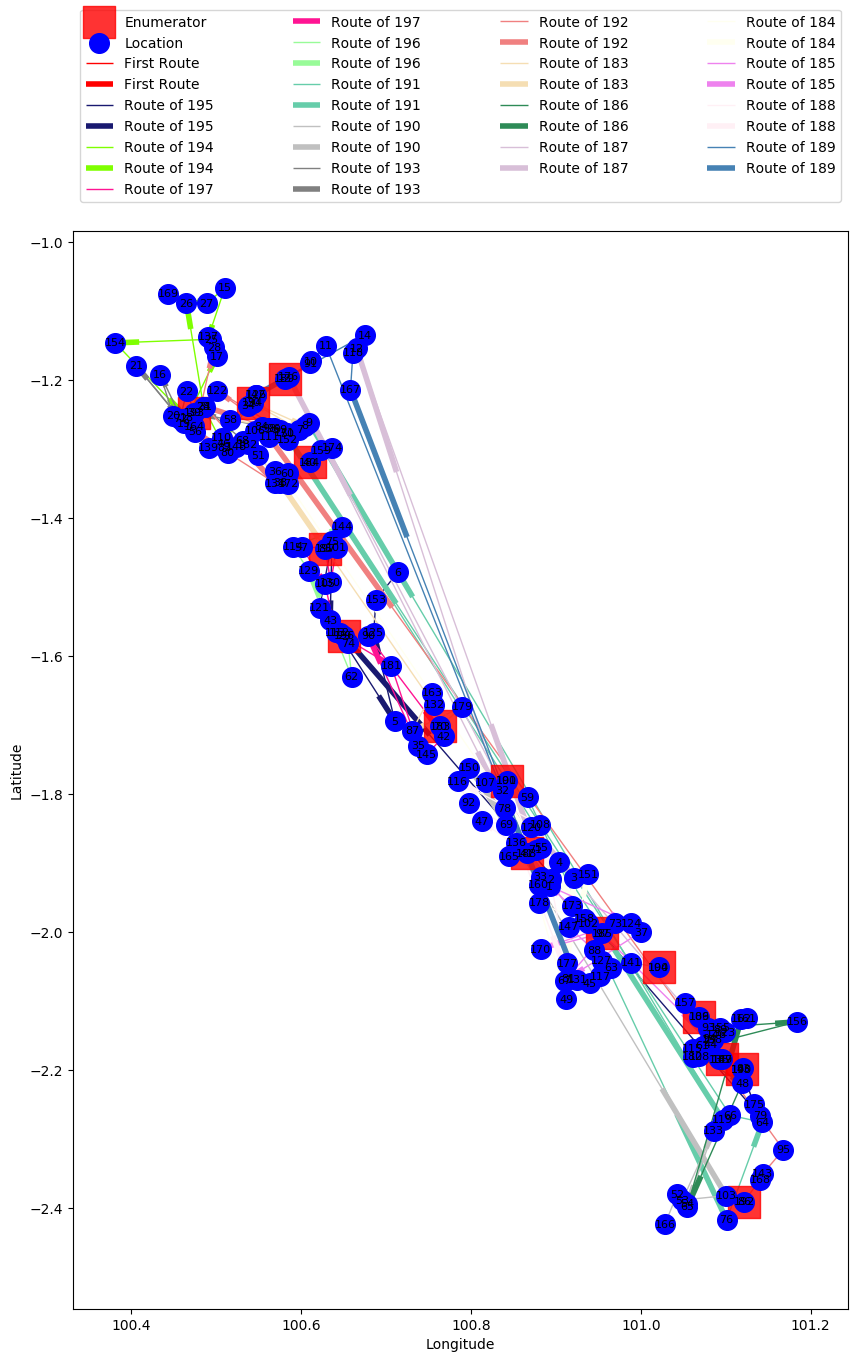
\includegraphics[width=\textwidth]{Resources/Images/test_result_normal_field_m15_n182_pubsub_coes}
%	\caption{Rute Hasil Pengujian Data Lapangan Pada MDVRP berbasis CoEAs dengan Publish/Subscribe}
%	\label{fig:test_result_normal_field_pubsub_coes}
%\end{figure}


%-----------------------------------------------------------------------------%
\subsubsection{Pengujian Kondisi \textit{Delay} dengan \textit{Service Time}}
\label{sssec:test-delay-service-time}
%-----------------------------------------------------------------------------%
Skenario pengujian kondisi \textit{delay} dimaksudkan untuk membandingkan program yang dijalankan pada kondisi terjadi hal-hal yang menghambat jalannya pencacahan. Pengujian ini digunakan sebagai cerminan kodisi lapangan dimana pada beberapa lokasi tidak terdapat koneksi yang stabil, sehingga untuk melakukan \textit{subscription} lokasi berikutnya perlu berpindah ke lokasi lain. Pengujian dilakukan sebanyak 7 (tujuh) kali, dimana masing-masing mencerminkan kondisi yang berbeda, yaitu:

\begin{enumerate}
	\item Pengujian dengan kode \textit{instance} d01 menggambarkan kondisi normal. Parameter yang digunakan pada \textit{instance} ini adalah sebagai berikut:
	\begin{itemize}
		\item Jumlah responden pada setiap segmen/blok sensus adalah 10 rumah tangga
		\item Rata-rata wawancara pada setiap rumah tangga 27,58 menit dengan standar deviasi 12,13 menit.
		\item Rata-rata waktu yang diperlukan untuk mendapatkan koneksi internet sebesar 5 menit dengan standar deviasi 3 menit.
	\end{itemize}
	\item Pengujian dengan kode \textit{instance} d02 menggambarkan kondisi dimana anggota rumah tangga sedikit dan relatif homogen, dengan koneksi internet relatif mudah didapatkan. Parameter yang digunakan pada \textit{instance} ini adalah sebagai berikut:
	\begin{itemize}
		\item Jumlah responden pada setiap segmen/blok sensus adalah 10 rumah tangga
		\item Rata-rata wawancara pada setiap rumah tangga 27,58 menit dengan standar deviasi 4,16 menit.
		\item Rata-rata waktu yang diperlukan untuk mendapatkan koneksi internet sebesar 5 menit dengan standar deviasi 3 menit.
	\end{itemize}
	\item Pengujian dengan kode \textit{instance} d03 menggambarkan kondisi dimana anggota rumah tangga sedikit dan relatif homogen, dengan koneksi internet secara umum sulit didapatkan. Parameter yang digunakan pada \textit{instance} ini adalah sebagai berikut:
	\begin{itemize}
		\item Jumlah responden pada setiap segmen/blok sensus adalah 10 rumah tangga
		\item Rata-rata wawancara pada setiap rumah tangga 27,58 menit dengan standar deviasi 4,16 menit.
		\item Rata-rata waktu yang diperlukan untuk mendapatkan koneksi internet sebesar 60 menit dengan standar deviasi 3 menit.
	\end{itemize}
	\item Pengujian dengan kode \textit{instance} d04 menggambarkan kondisi dimana anggota rumah tangga banyak dan relatif homogen, dengan koneksi internet relatif mudah didapatkan. Parameter yang digunakan pada \textit{instance} ini adalah sebagai berikut:
	\begin{itemize}
		\item Jumlah responden pada setiap segmen/blok sensus adalah 10 rumah tangga
		\item Rata-rata wawancara pada setiap rumah tangga 71,58 menit dengan standar deviasi 12,16 menit.
		\item Rata-rata waktu yang diperlukan untuk mendapatkan koneksi internet sebesar 5 menit dengan standar deviasi 3 menit.
	\end{itemize}
	\item Pengujian dengan kode \textit{instance} d05 menggambarkan kondisi dimana anggota rumah tangga banyak dan relatif homogen, dengan koneksi internet secara umum sulit didapatkan. Parameter yang digunakan pada \textit{instance} ini adalah sebagai berikut:
	\begin{itemize}
		\item Jumlah responden pada setiap segmen/blok sensus adalah 10 rumah tangga
		\item Rata-rata wawancara pada setiap rumah tangga 71,58 menit dengan standar deviasi 12,16 menit.
		\item Rata-rata waktu yang diperlukan untuk mendapatkan koneksi internet sebesar 60 menit dengan standar deviasi 3 menit.
	\end{itemize}
	\item Pengujian dengan kode \textit{instance} d06 menggambarkan kondisi dimana rata-rata anggota rumah tangga sedikit tetapi memiliki variasi tinggi, dengan koneksi internet secara umum sulit didapatkan. Parameter yang digunakan pada \textit{instance} ini adalah sebagai berikut:
	\begin{itemize}
		\item Jumlah responden pada setiap segmen/blok sensus adalah 10 rumah tangga
		\item Rata-rata wawancara pada setiap rumah tangga 27,58 menit dengan standar deviasi 25,16 menit.
		\item Rata-rata waktu yang diperlukan untuk mendapatkan koneksi internet sebesar 60 menit dengan standar deviasi 3 menit.
	\end{itemize}
	\item Pengujian dengan kode \textit{instance} d07 menggambarkan kondisi dimana jarak antar rumah tangga jauh, rata-rata anggota rumah tangga banyak dan memiliki variasi tinggi, dan koneksi internet secara umum sulit didapatkan. Parameter yang digunakan pada \textit{instance} ini adalah sebagai berikut:
	\begin{itemize}
		\item Jumlah responden pada setiap segmen/blok sensus adalah 10 rumah tangga
		\item Rata-rata wawancara pada setiap rumah tangga 71,58 menit dengan standar deviasi 25,65 menit.
		\item Rata-rata waktu tempuh antar rumah tangga 30,45 menit dengan standar deviasi 22,12 menit.
		\item Rata-rata waktu yang diperlukan untuk mendapatkan koneksi internet sebesar 60 menit dengan standar deviasi 3 menit.
	\end{itemize}
\end{enumerate}


Dari hasil simulasi, diperoleh rute untuk masing-masing \textit{instance} sebagaimana digambarkan pada \hyperref[ch:test_result_delay]{Lampiran 2}. \textit{Total time} untuk masing-masing rute dapat dilihat pada \autoref{tbl:test_result_delay}. Hasil pengujian pada tabel \autoref{tbl:test_result_delay} menunjukkan hasil yang relatif sama dan sekaligus menegaskan kembali kesimpulan yang telah diperoleh pada skenario pengujian sebelumnya, yakni sistem usulan lebih efisien dibandingkan sistem pembanding. \autoref{fig:test_result_delay_total_time} dan \autoref{fig:test_result_delay_standard_deviation} menggambarkan perbandingan hasil pengujian dari 7 \textit{instance}.


\begin{longtable}[!]{l|rrrr}
	\caption{Hasil Pengujian Kondisi Delay Dengan \textit{Service Time} pada Data Lapangan}
	\label{tbl:test_result_delay}\\
	\toprule
	\textit{Instance} & \MyHead{2.5cm}{Total Waktu CoES MDVRP (det)} & \MyHead{2.5cm}{Total Waktu CoES MDVRP + Pub/Sub (det)} & \MyHead{2.5cm}{Stdev Waktu CoES MDVRP (det)} & \MyHead{2.5cm}{Stdev Waktu CoES MDVRP + Pub/Sub (det)} \\ 
	\midrule
	\endfirsthead
	\toprule
	\textit{Instance} & \MyHead{2.5cm}{Total Waktu CoES MDVRP (det)} & \MyHead{2.5cm}{Total Waktu CoES MDVRP + Pub/Sub (det)} & \MyHead{2.5cm}{Stdev Waktu CoES MDVRP (det)} & \MyHead{2.5cm}{Stdev Waktu CoES MDVRP + Pub/Sub (det)} \\ 
	\midrule
	\endhead
	\bottomrule
	\endfoot
	d01 & \textbf{3,126,361.44} & 3,532,199.80 & 85,427.10 & \textbf{16,565.69} \\
	d02 & \textbf{3,107,775.85} & 3,743,549.71 & 84,873.08 & \textbf{13,445.49} \\
	d03 & \textbf{3,085,573.84} & 3,901,417.79 & 83,869.48 & \textbf{21,175.88} \\
	d04 & \textbf{7,937,588.57} & 8,262,690.25 & 204,164.67 & \textbf{21,147.45} \\
	d05 & \textbf{7,903,175.28} & 8,820,620.43 & 210,500.85 & \textbf{26,542.12} \\
	d06 & \textbf{3,083,461.58} & 4,019,585.94 & 84,959.86 & \textbf{22,071.07} \\
	d07 & \textbf{10,792,753.12} & 11,590,204.96 & 280,996.99 & \textbf{29,048.13} \\
\end{longtable}


\begin{figure}[H]
	\centering
	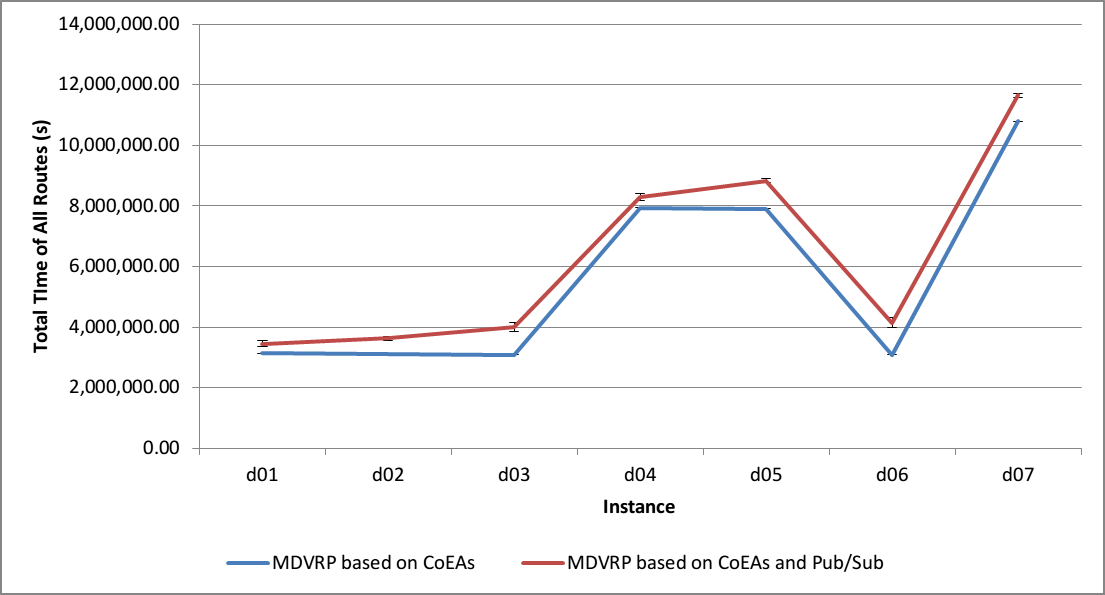
\includegraphics[width=\textwidth]{Resources/Images/test_result_delay_total_time}
	\caption{Perbandingan Waktu Total dari 7 \textit{Instance}}
	\label{fig:test_result_delay_total_time}
\end{figure}


\begin{figure}[H]
	\centering
	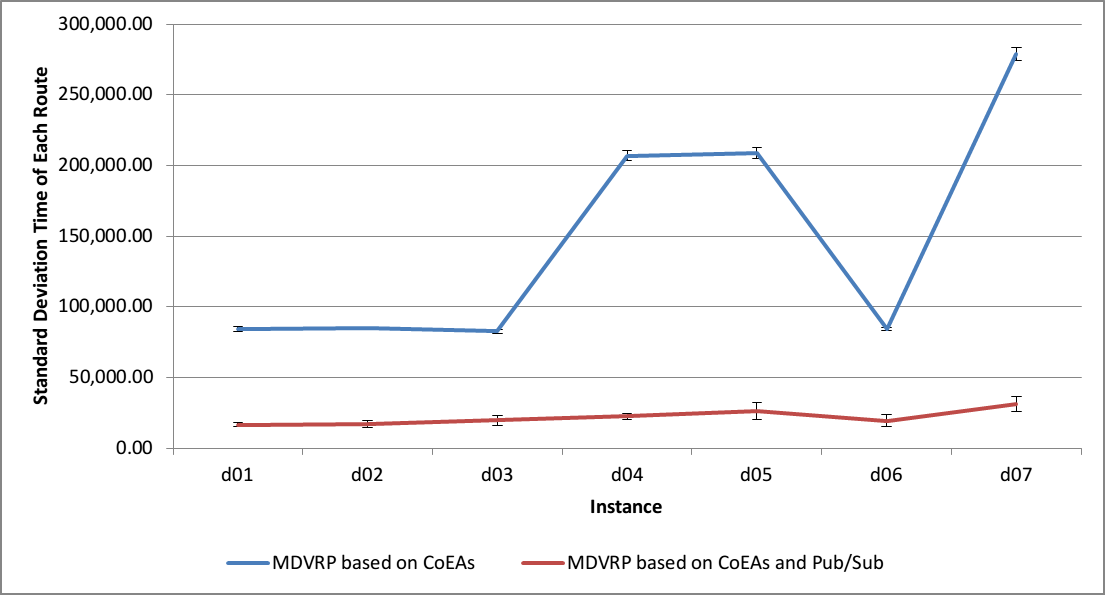
\includegraphics[width=\textwidth]{Resources/Images/test_result_delay_standard_deviation}
	\caption{Perbandingan Standar Deviasi Waktu dari 7 \textit{Instance}}
	\label{fig:test_result_delay_standard_deviation}
\end{figure}


%%-----------------------------------------------------------------------------%
%\subsubsection{Pengujian Kondisi Pencacah Berhenti dengan \textit{Service Time}}
%\label{sssec:test-quit-service-time}
%%-----------------------------------------------------------------------------%


%\begin{longtable}[!]{l|rrrr}
%	\caption{Hasil Pengujian Kondisi Normal Pada Data Cordeau Dengan \textit{Service Time}}
%	\label{tbl:test_result_10_cordeau_tw}\\
%	\toprule
%	\textit{Instance} & \MyHead{2.5cm}{Total Waktu CoES MDVRP (det)} & \MyHead{2.5cm}{Total Waktu CoES MDVRP + Pub/Sub (det)} & \MyHead{2.5cm}{Stdev Waktu CoES MDVRP (det)} & \MyHead{2.5cm}{Stdev Waktu CoES MDVRP + Pub/Sub (det)} \\ 
%	\midrule
%	\endfirsthead
%	\toprule
%	\textit{Instance} & \MyHead{2.5cm}{Total Waktu CoES MDVRP (det)} & \MyHead{2.5cm}{Total Waktu CoES MDVRP + Pub/Sub (det)} & \MyHead{2.5cm}{Stdev Waktu CoES MDVRP (det)} & \MyHead{2.5cm}{Stdev Waktu CoES MDVRP + Pub/Sub (det)} \\ 
%	\midrule
%	\endhead
%	\bottomrule
%	\endfoot
%	q01 &  & 3,464,733.76 &  & 37,997.03 \\
%	q02 &  & 3,635,752.13 &  & 68,239.51 \\
%	q03 &  & 3,611,394.03 &  & 98,900.33 \\
%\end{longtable}


%%-----------------------------------------------------------------------------%
%\subsubsection{Pengujian Kondisi \textit{Packet Loss} pada Jaringan dengan \textit{Service Time}}
%%-----------------------------------------------------------------------------%
%Skenario pengujian kondisi \textit{packet loss} pada jaringan dimaksudkan untuk membandingkan program yang dijalankan pada kondisi dimana terjadi \textit{packet loss}. Pengujian ini digunakan sebagai cerminan kodisi lapangan dimana pada beberapa lokasi tidak terdapat koneksi yang stabil. Pengujian akan dilakukan satu kali untuk data lapangan. Sementara data \textit{service time} digenerate secara random dengan mengikuti komposisi dari \citep{sudman_time_1965} sebagaimana dijelaskan pada \autoref{ssec:test-normal-service-time}.
%
%
%Pada pengujian ini juga akan digunakan sebuah software \textit{$3^{rd}$}, yaitu Pumba \citep{1013821358660176_pumba_2016} untuk meng-emulasi-kan \textit{packet loss}. Nilai \textit{Packet loss} yang digunakan adalah 10\% dari packet yang lewat yang dipilih secara random. Langkah-langkah yang dilakukan dalam konfigurasi Pumba adalah seperti pada \autoref{fig:test-flowchart-normal-global-netem}.
%
%
%\begin{figure}[!]
%	\centering
%	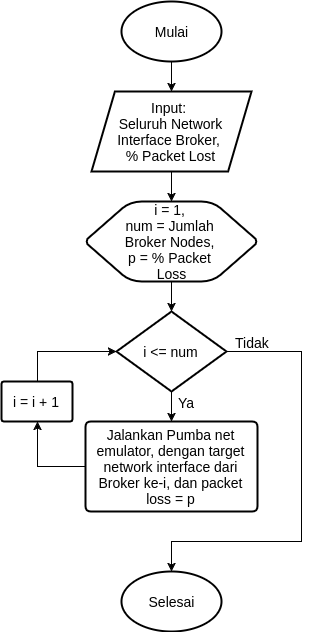
\includegraphics[width=0.5\textwidth]{Resources/Images/test-flowchart-normal-global-netem-packet-loss}
%	\caption{Flowchart Setup Pumba Net Emulator}
%	\label{fig:test-flowchart-normal-global-netem-packet-loss}
%\end{figure}
%
%
%Berdasarkan hasil pengujian, diperoleh hasil sebagaimana \autoref{tbl:test_result_packet_loss_field_coes} untuk algoritma MDVRP berbasis CoEAs tanpa mekanisme Publish/Subscribe, dan \autoref{tbl:test_result_packet_loss_field_pubsub_coes} untuk algoritma MDVRP berbasis CoEAs dengan mekanisme Publish/Subscribe. Sementara \autoref{fig:test_result_packet_loss_field_comparison} menggambarkan rute yang diperoleh untuk masing-masing program.
%
%
%Berdasarkan \autoref{fig:test_result_packet_loss_field_comparison}, diperoleh hasil bahwasannya \textbf{total waktu} yang diperoleh dengan menggunakan sistem MDVRP berbasis CoEAs dan Publish/Subscribe lebih buruk 12,79 persen  dibandingkan dengan program usulan. Akan tetapi dari sisi \textbf{standar deviasi} dari keseluruhan rute diperoleh hasil metode CoEAs yang dikombinasikan dengan Publish/Subscribe menghasilkan angka yang lebih baik 36,14 persen, yang artinya total waktu dari seluruh rute lebih merata.
%
%
%\begin{longtable}[!]{lp{8cm}r}
%	\caption{Hasil Pengujian Kondisi \textit{Packet Loss}, MDVRP berbasis CoEAs}
%	\label{tbl:test_result_packet_loss_field_coes}\\
%	\toprule
%	\textit{Vehicle} & Rute & Waktu Total\\ 
%	\midrule
%	\endfirsthead
%	\toprule
%	\textit{Vehicle} & Rute & Waktu Total\\ 
%	\midrule
%	\endhead
%	\bottomrule
%	\endfoot
%	183 & 70-179-87-163-132-5-35-145-42 & 170,349.48 \\
%	184 & 159-174-60-36-99-98-171-50-9-7-8-152-111-51-40-172-38-134 & 331,759.24 \\
%	185 & 127-88-147-173-158-102-124-37-73-97 & 184,993.17 \\
%	186 & 157-93-94-146-155-123-162-161-156-89-138-77-44-109 & 254,089.65 \\
%	187 & 149-135-61-115-180-128 & 109,758.28 \\
%	188 & 41-165-47-78-69-108-120-136-71-55-4-33-178-160-1-151-3-2 & 337,519.02 \\
%	189 & 13-91-10-11-14-12-118-167-176 & 168,298.11 \\
%	190 & 104-141-63-117-45-131-81-177-170-67-49 & 193,952.81 \\
%	191 & 100-107-92-116-150-32-59 & 134,042.73 \\
%	192 & 86-168-143-95-76-103-53-52-166-65-54 & 211,842.84 \\
%	193 & 164-139-56-18-72-19-20-22-21-16-39-24-23-17-28-137-26-169-154-27-15-25-122-31 & 451,562.34 \\
%	194 & 142-126-30-58-110-46-82-80-148-106-96-84-68-182-34 & 275,108.47 \\
%	195 & 83-140-175-79-64-133-119-66-48 & 160,970.13 \\
%	196 & 29-112-113-43-121-74-90-125-153-6-181-62 & 220,804.42 \\
%	197 & 85-129-130-105-114-57-144-75-101 & 168,014.48 \\
%\end{longtable}
%
%
%\begin{longtable}[!]{lp{8cm}r}
%	\caption{Hasil Pengujian Kondisi \textit{Packet Loss}, MDVRP berbasis CoEAs dan Publish/Subscribe}
%	\label{tbl:test_result_packet_loss_field_pubsub_coes}\\
%	\toprule
%	\textit{Vehicle} & Rute & Waktu Total\\ 
%	\midrule
%	\endfirsthead
%	\toprule
%	\textit{Vehicle} & Rute & Waktu Total\\ 
%	\midrule
%	\endhead
%	\bottomrule
%	\endfoot
%	183 & 70-179-87-163-5-132-35-42-150-145-116-92-181 & 248,263.36 \\
%	184 & 159-38-36-134-171-98-99-50-152-51-9-111-60-7-8-172-40-174 & 337,070.24 \\
%	185 & 127-88-93-147-89-123-162-161-156-155-133-48 & 227,271.63 \\
%	186 & 157-109-128-146-138-94-77-44-61-158-115-67-180-97-170 & 293,534.49 \\
%	187 & 149-135-136-47-69-108-78-55-4-1-33-2-160-178-102-3-151 & 327,824.92 \\
%	188 & 41-165-71-120-45-173-11-73-176-166-118 & 292,972.01 \\
%	189 & 13-91-63-10-124-177-37-53-52-65 & 233,724.33 \\
%	190 & 104-141-32-117-131-81-76-49-103-56-21-16 & 271,621.19 \\
%	191 & 100-107-143-59-64-18-66-72-119-20 & 294,953.97 \\
%	192 & 86-168-17-95-137-26-27-15-25-169-154 & 257,340.44 \\
%	193 & 164-31-139-122-24-39-23-28-22-96-19-68-84-167 & 272,916.02 \\
%	194 & 142-30-34-126-46-182-148-58-106-80-82-12-110-14 & 266,327.10 \\
%	195 & 83-140-113-175-74-79-43-54-62 & 245,755.86 \\
%	196 & 29-112-75-121-105-129-130-90-125-153-6 & 206,966.83 \\
%	197 & 85-114-144-101-57 & 91,540.79 \\
%\end{longtable}
%
%
%\begin{longtable}[!]{lrr}
%	\caption{Komparasi Hasil Pengujian Kondisi \textit{Packet Loss} Dengan Data Lapangan}
%	\label{tbl:test_result_packet_loss_field_comparison}\\
%	\toprule
%	\textit{Parameter} & CoEAs MDVRP  & Pub/Sub CoEAS MDVRP\\ 
%	\midrule
%	\endfirsthead
%	\toprule
%	\textit{Parameter} & CoEAs MDVRP  & Pub/Sub CoEAS MDVRP\\ 
%	\midrule
%	\endhead
%	\bottomrule
%	\endfoot
%	Total Waktu & \textbf{3,373,065.19} & 3,868,083.19\\
%	Rata-rata & \textbf{224,871.01} & 257,872.21\\
%	Standar Deviasi & 88,167.80 & \textbf{56,301.47}\\
%\end{longtable}
%
%
%\begin{figure}[H]
%	\centering
%	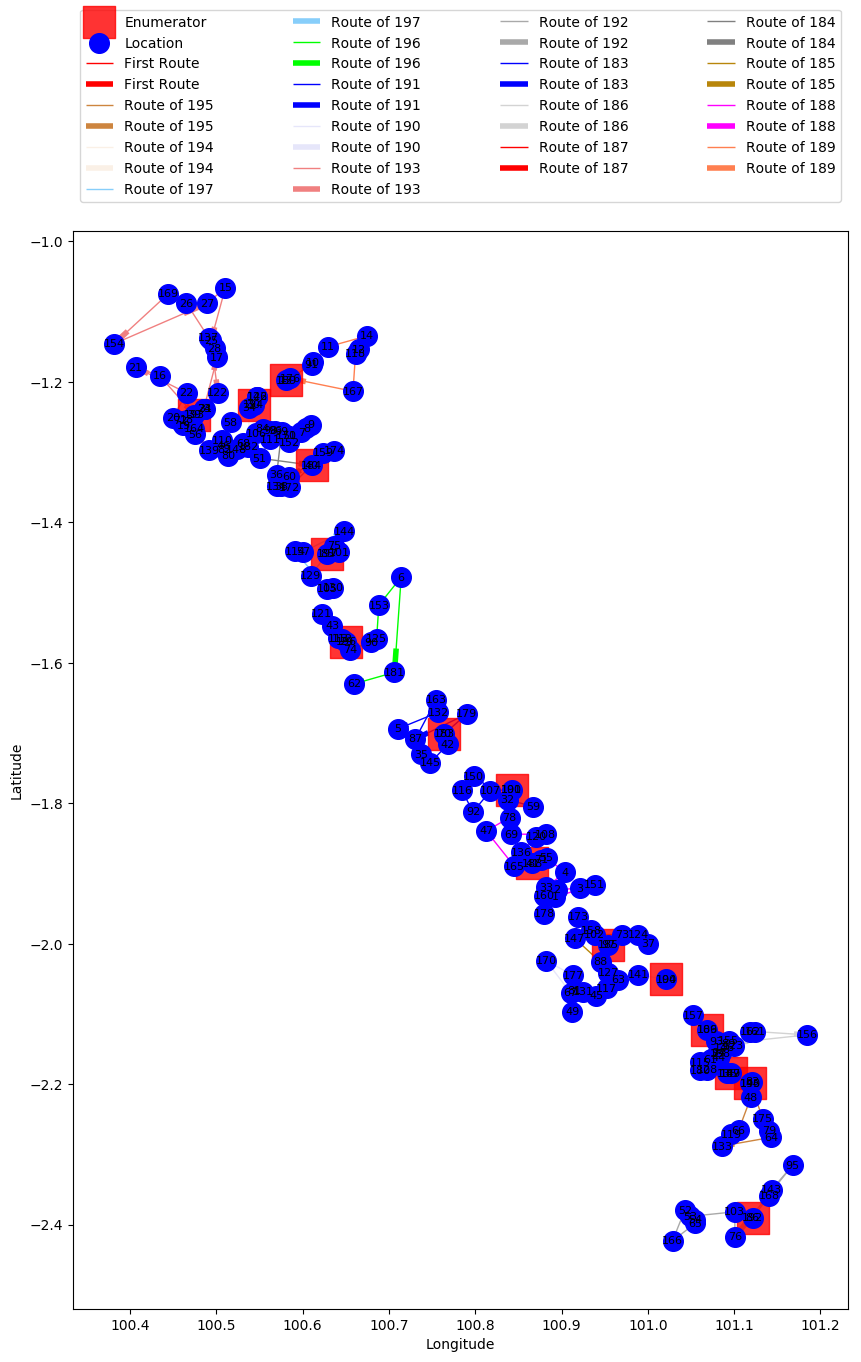
\includegraphics[width=\textwidth]{Resources/Images/test_result_normal_field_m15_n182_packet_loss_coes}
%	\caption{Rute Hasil Pengujian Kondisi \textit{Packet Loss} Data Lapangan Pada MDVRP berbasis CoEAs}
%	\label{fig:test_result_packet_loss_field_coes}
%\end{figure}
%
%
%\begin{figure}[H]
%	\centering
%	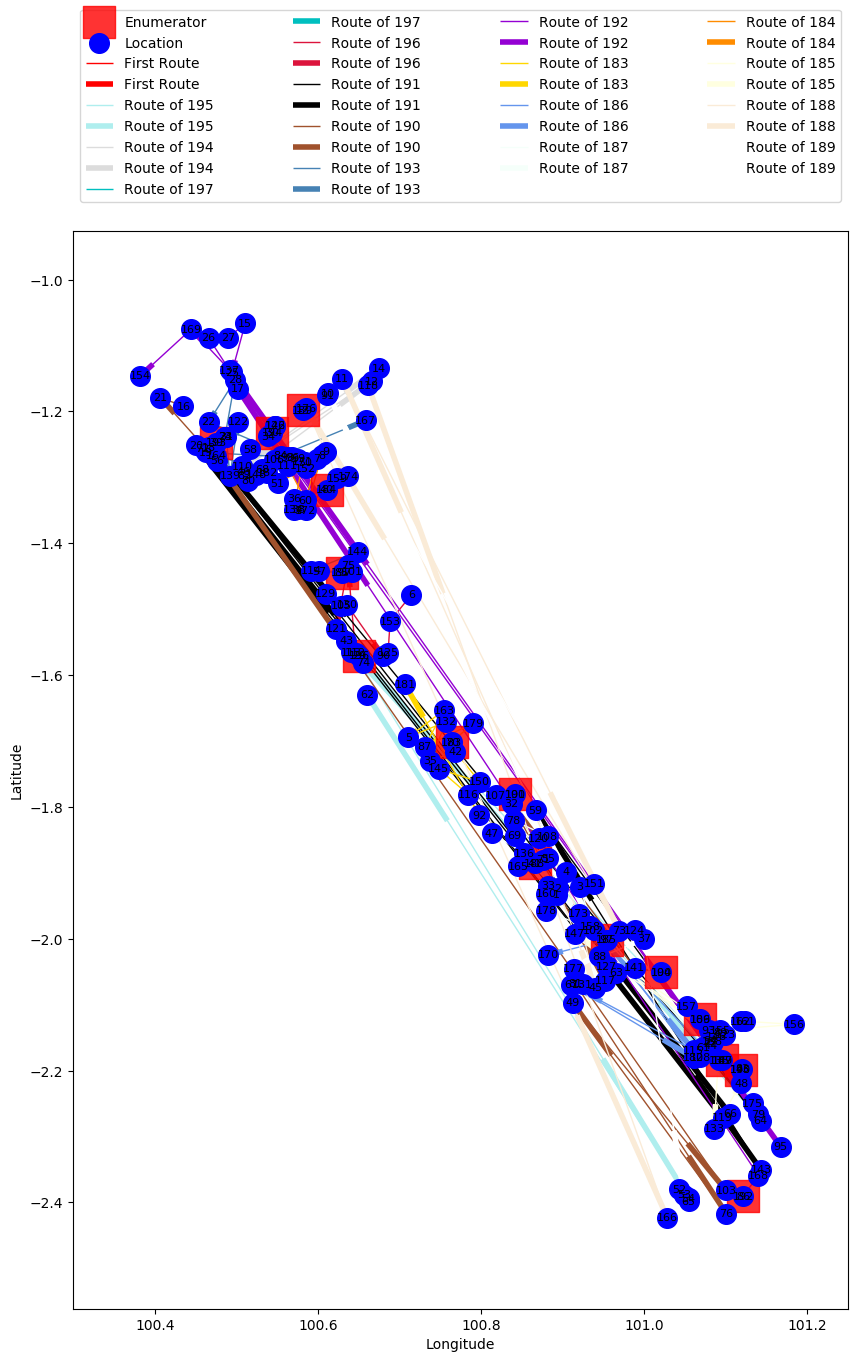
\includegraphics[width=\textwidth]{Resources/Images/test_result_normal_field_m15_n182_packet_loss_pubsub_coes}
%	\caption{Rute Hasil Pengujian Kondisi \textit{Packet Loss} Data Lapangan Pada MDVRP berbasis CoEAs dengan Publish/Subscribe}
%	\label{fig:test_result_packet_loss_field_pubsub_coes}
%\end{figure}


%%-----------------------------------------------------------------------------%
%\subsubsection{Pengujian Kondisi Pencacah Berhenti}
%%-----------------------------------------------------------------------------%
%Skenario pengujian kondisi pencacah berhenti dimaksudkan untuk membandingkan program yang dijalankan pada kondisi dimana satu atau lebih pencacah berhenti pada saat pencacahan tengah berlangsung. Pengujian akan dilakukan satu kali untuk data lapangan. Pada pengujian ini sebuah program \textit{client} dirancang sebagai simulator.
%
%
%\begin{figure}[!]
%    \centering
%    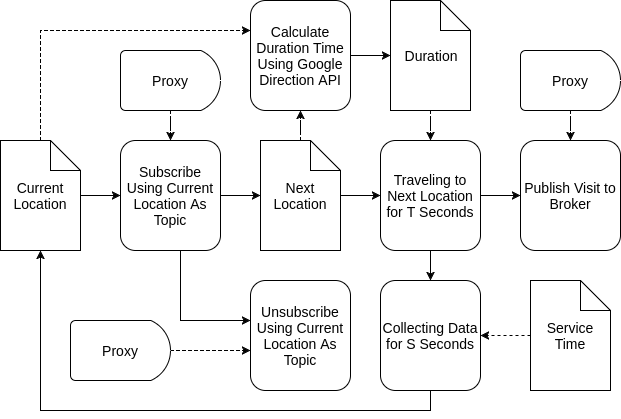
\includegraphics[width=\textwidth]{Resources/Images/client-algorithm-enumerator-quit-field}
%    \caption{\textit{Flowchart} pada \textit{Client Simulator} Kondisi Pencacah Berhenti}
%    \label{fig:client-algorithm-enumerator-quit-field}
%\end{figure}
%
%
%Langkah-langkah yang diimplementasikan pada program \textit{client}, sebagaimana ilustrasi Gambar \ref{fig:client-algorithm-enumerator-quit-field}, adalah sebagai berikut:
%
%\begin{enumerate}
%\item Buat koneksi dengan \textit{message broker}, 
%\item Lakukan \textit{subscription} dengan topik \textit{current location}, 
%\item Setelah sebuah \textit{message} diterima, dimana \textit{message} dari \textit{broker} merupakan \textit{next location}, kalkulasi waktu tempuh antara \textit{current location} dengan \textit{next location},
%\item Simulasikan perjalanan ke lokasi dengan \textit{sleep},
%\item Buat notifikasi terhadap broker atas perubahan \textit{current location}, 
%\item Generate \textit{service time}, mengikuti distribusi normal, 
%\item Simulasikan pencacahan dengan \textit{sleep}, 
%\item Hentikan beberapa proses, 
%\item Ulangi lagi dari langkah pertama.
%\end{enumerate}
%
%
%Pada pengujian ini, disimulasikan bahwasannya pencacah 1302110003 berhenti setelah 150000 detik, 1302101005 setelah 360000 detik, 1302012003 setelah 180000 detik, dan 1302080006 setelah 300000 detik. Tabel \ref{tbl:test_result_enumerator_quit_field_pubsub_coes} menunjukkan hasil simulasi dan waktu total untuk masing-masing pencacah. Ketika rute dari keempat pencacah tersebut dikeluarkan dari penghitungan standar deviasi, maka sebagaimana Tabel \ref{tbl:test_result_enumerator_quit_field} diperoleh .
%
%\begin{longtable}[!]{lp{8cm}r}
%	\caption{Hasil Pengujian Kondisi Pencacah Berhenti (Lapangan), CoEAs}
%	\label{tbl:test_result_enumerator_quit_field_coes}\\
%	\toprule
%		\textit{Vehicle} & Rute & Waktu Total\\ 
%	\midrule
%	\endfirsthead
%	\toprule
%		\textit{Vehicle} & Rute & Waktu Total\\ 
%	\midrule
%	\endhead
%	\bottomrule
%	\endfoot
%		
%\end{longtable}
%
%
%\begin{longtable}[!]{lp{8cm}r}
%	\caption{Hasil Pengujian Kondisi Pencacah Berhenti (Lapangan), CoEAs + Publish/Subscribe}
%	\label{tbl:test_result_enumerator_quit_field_pubsub_coes}\\
%	\toprule
%		\textit{Vehicle} & Rute & Waktu Total\\ 
%	\midrule
%	\endfirsthead
%	\toprule
%		\textit{Vehicle} & Rute & Waktu Total\\ 
%	\midrule
%	\endhead
%	\bottomrule
%	\endfoot
%		1302011008 & 1302011008-1302011008-1302011010-1302011001-1302012005-1302011007-1302011009-1302011005-1302011006-1302011002-1302011004-1302011003-1302090007-1302090015-1302110002-1302110013-1302110006 & 407401.10 \\
%		1302040002 & 1302040002-1302040002-1302040016-1302040004-1302040005-1302040006-1302040015-1302040007-1302040003-1302040009-1302040013-1302040008-1302090013 & 306233.49 \\
%		1302012003 & 1302012003-1302012008-1302012003-1302012001-1302012006-1302012002-1302012004-1302012010 & 169070.15 \\
%		1302060005 & 1302060005-1302060005-1302060009-1302060006-1302060008-1302060007-1302060001-1302060004-1302050010-1302050009-1302060003-1302012009-1302100016-1302090010 & 345013.89 \\
%		1302020006 & 1302020006-1302020006-1302020016-1302020015-1302021002-1302021006-1302020017-1302031005 & 171648.83 \\
%		1302080006 & 1302080006-1302080006-1302080007-1302080008-1302080002-1302080001-1302080004-1302080009-1302070012-1302070003-1302080003-1302080005 & 269836.91 \\
%		1302021005 & 1302021005-1302021005-1302021001-1302020011-1302020009-1302020001-1302020010-1302021003-1302021008-1302021010-1302021007-1302021009-1302021004-1302110012 & 335580.21 \\
%		1302100002 & 1302100002-1302100002-1302100003-1302100013-1302100009-1302100001-1302100005-1302110023-1302110021-1302110022-1302110008-1302110007-1302110020-1302110018-1302110009-1302110003-1302110010-1302110005 & 428783.15 \\
%		1302101005 & 1302101005-1302101005-1302100010-1302101002-1302100014-1302100011-1302101003-1302101001-1302100006-1302100004-1302100012-1302100007-1302100017-1302101004 & 327886.72 \\
%		1302110003 & 1302110003-1302110019-1302110004-1302110001-1302110011-1302110017-1302110016 & 147061.67 \\
%		1302090004 & 1302090004-1302090008-1302090002-1302090005-1302090004-1302090012-1302090014-1302090020-1302090019-1302090001-1302090017-1302090018-1302090016-1302110014-1302101006-1302090011 & 368625.31 \\
%		1302030005 & 1302030005-1302030005-1302030014-1302030006-1302030009-1302030004-1302030012-1302030003-1302031004-1302030010-1302030002-1302031003-1302020005-1302020003-1302100015-1302100008 & 382133.70 \\
%		1302070006 & 1302070006-1302070006-1302070002-1302070011-1302070005-1302070008-1302070009-1302070010-1302070007-1302070001-1302070004-1302060002-1302110015 & 299606.48 \\
%		1302050007 & 1302050007-1302050007-1302050008-1302050002-1302050006-1302050004-1302050001-1302050003-1302050005-1302040001-1302040012-1302012007-1302090006-1302090009-1302090003 & 369932.48 \\
%		1302031005 & 1302031005-1302031001-1302031006-1302031008-1302040011-1302031009-1302031010-1302040010-1302031007-1302030001-1302031002-1302040014 & 278953.18 \\
%\end{longtable}
%
%
%\begin{longtable}[!]{lrr}
%	\caption{Komparasi CoEAs dan Publish/Subscribe + CoEAs pada Data Lapangan}
%	\label{tbl:test_result_enumerator_quit_field}\\
%	\toprule
%		Ukuran & CoEAs & CoEAs + Publish/Subscribe\\ 
%	\midrule
%	\endfirsthead
%	\toprule
%		Ukuran & CoEAs & CoEAs + Publish/Subscribe\\ 
%	\midrule
%	\endhead
%	\bottomrule
%	\endfoot
%		Total Waktu & 4448989.67 & 4607767.28\\
%		Rata-rata & 296599.31 & 307184.49\\
%		Standar Deviasi & 119720.84 & 84126.97\\
%\end{longtable}

